% Created with jtex v.1.0.20
\documentclass{article}
\usepackage{hyperref}
\usepackage{datetime}
\usepackage{graphicx}
\usepackage{natbib}
\bibliographystyle{abbrvnat}

%%%%%%%%%%%%%%%%%%%%%%%%%%%%%%%%%%%%%%%%%%%%%%%%%%
%%%%%%%%%%%%%%%%%%%%  imports  %%%%%%%%%%%%%%%%%%%
\usepackage{booktabs}
\usepackage{framed}
\usepackage{url}
%%%%%%%%%%%%%%%%%%%%%%%%%%%%%%%%%%%%%%%%%%%%%%%%%%


% colors for hyperlinks
\hypersetup{colorlinks=true, allcolors=blue}

\newcommand{\logo}{
  \href{https://curvenote.com}{
\includegraphics[width=2cm]{curvenote.png}}
}

\title{4. Psychoacoustics}

\author{MUS2640 \and University of Oslo}

\newdate{articleDate}{11}{4}{2026}
\date{\displaydate{articleDate}}

\begin{document}
\maketitle
\begin{center}\logo\end{center}


This week we will explore the field of \textit{\href{https://en.wikipedia.org/wiki/Psychoacoustics}{psychoacoustics}}, the study of how humans perceive and interpret sound, bridging the gap between physical sound properties and subjective auditory experiences. Psychoacoustics examines the psychological and physiological responses associated with sound, including how we detect, differentiate, and interpret auditory stimuli. It seeks to answer questions such as: Why do some sounds seem louder than others, even if they have the same physical intensity? How do we distinguish between different musical instruments playing the same note? What makes certain sounds pleasant or unpleasant? This will form the foundation for more detailed investigations of ``vertical'' and ``horizontal'' sound perception in the coming weeks.

\section{Introduction to Psychoacoustics}

Psychoacoustics is a specialized area within the broader field of \textit{\href{https://en.wikipedia.org/wiki/Psychophysics}{psychophysics}}, which studies the relationships between physical stimuli and the sensations and perceptions they produce. While psychophysics investigates general principles of sensory perception across all senses, psychoacoustics focuses specifically on hearing. Both fields use experimental methods to quantify how changes in physical properties (like frequency, intensity, or duration) correspond to changes in perception (such as pitch, loudness, or timbre), helping to bridge the gap between objective measurements and subjective experience.

Psychoacoustics explores the relationship between the measurable, physical properties of sound (such as frequency, amplitude, and harmonic relationships) and the way these sounds are perceived by the human ear and brain (such as pitch, loudness, and timbre). Insights from psychoacoustics are applied in audio engineering, music production, hearing aid design, and the development of audio codecs (such as MP3), which exploit perceptual limitations to compress audio data efficiently.

The roots of psychoacoustics can be traced back to the 19th century, with foundational work by scientists such as \href{https://en.wikipedia.org/wiki/Hermann\_von\_Helmholtz}{Hermann von Helmholtz} (1821--1894), who investigated the sensations of tone and the physical basis of music. Later, \href{https://en.wikipedia.org/wiki/Stanley\_Smith\_Stevens}{S. S. Stevens}  (1906--1973) contributed to the development of psychophysical scaling, introducing methods to quantify the relationship between stimulus and perception (e.g., the Stevens' Power Law for loudness perception). Over time, psychoacoustics has evolved into a multidisciplinary field, integrating insights from physics, psychology, neuroscience, and engineering.

How does psychoacoustics relate to auditory \textit{perception} and \textit{cognition}? Psychoacoustics forms the scientific foundation for understanding how we perceive and interpret sound. Auditory perception encompasses the processes by which the ear and brain detect, analyze, and make sense of acoustic signals---transforming vibrations in the air into meaningful experiences such as speech, music, or environmental sounds. Psychoacoustics explains why certain sounds are perceived as louder, higher, or more pleasant, and how we can distinguish between different sources in complex auditory scenes.

Cognition involves higher-level mental functions such as attention, memory, learning, and decision-making. While psychoacoustics focuses on the sensory and perceptual mechanisms of hearing, cognition shapes how we interpret, remember, and respond to sounds. For example, cognitive processes help us focus on a single voice in a noisy room (the ``cocktail party effect''), recognize familiar melodies, or associate sounds with emotions and memories. Together, psychoacoustics and auditory cognition provide a comprehensive understanding of how we experience and interact with the world of sound.

\section{The Human Auditory System}

The human ear is a remarkably complex organ that enables us to detect sounds and maintain our sense of balance. It is divided into three main sections: the \textit{outer ear}, \textit{middle ear}, and \textit{inner ear}. Each part plays a distinct and crucial role in the auditory process.

\subsection{The outer ear}

The \textit{\href{https://en.wikipedia.org/wiki/Outer\_ear}{outer ear}} consists of the visible part called the \textit{pinna} and the \textit{ear canal}. Its primary function is to collect sound waves from the environment and funnel them toward the \textit{eardrum} (sometimes call the \textit{tympanic membrane}). The unique shape of the pinna helps us localize the direction of sounds. When sound waves reach the eardrum, they cause it to vibrate.

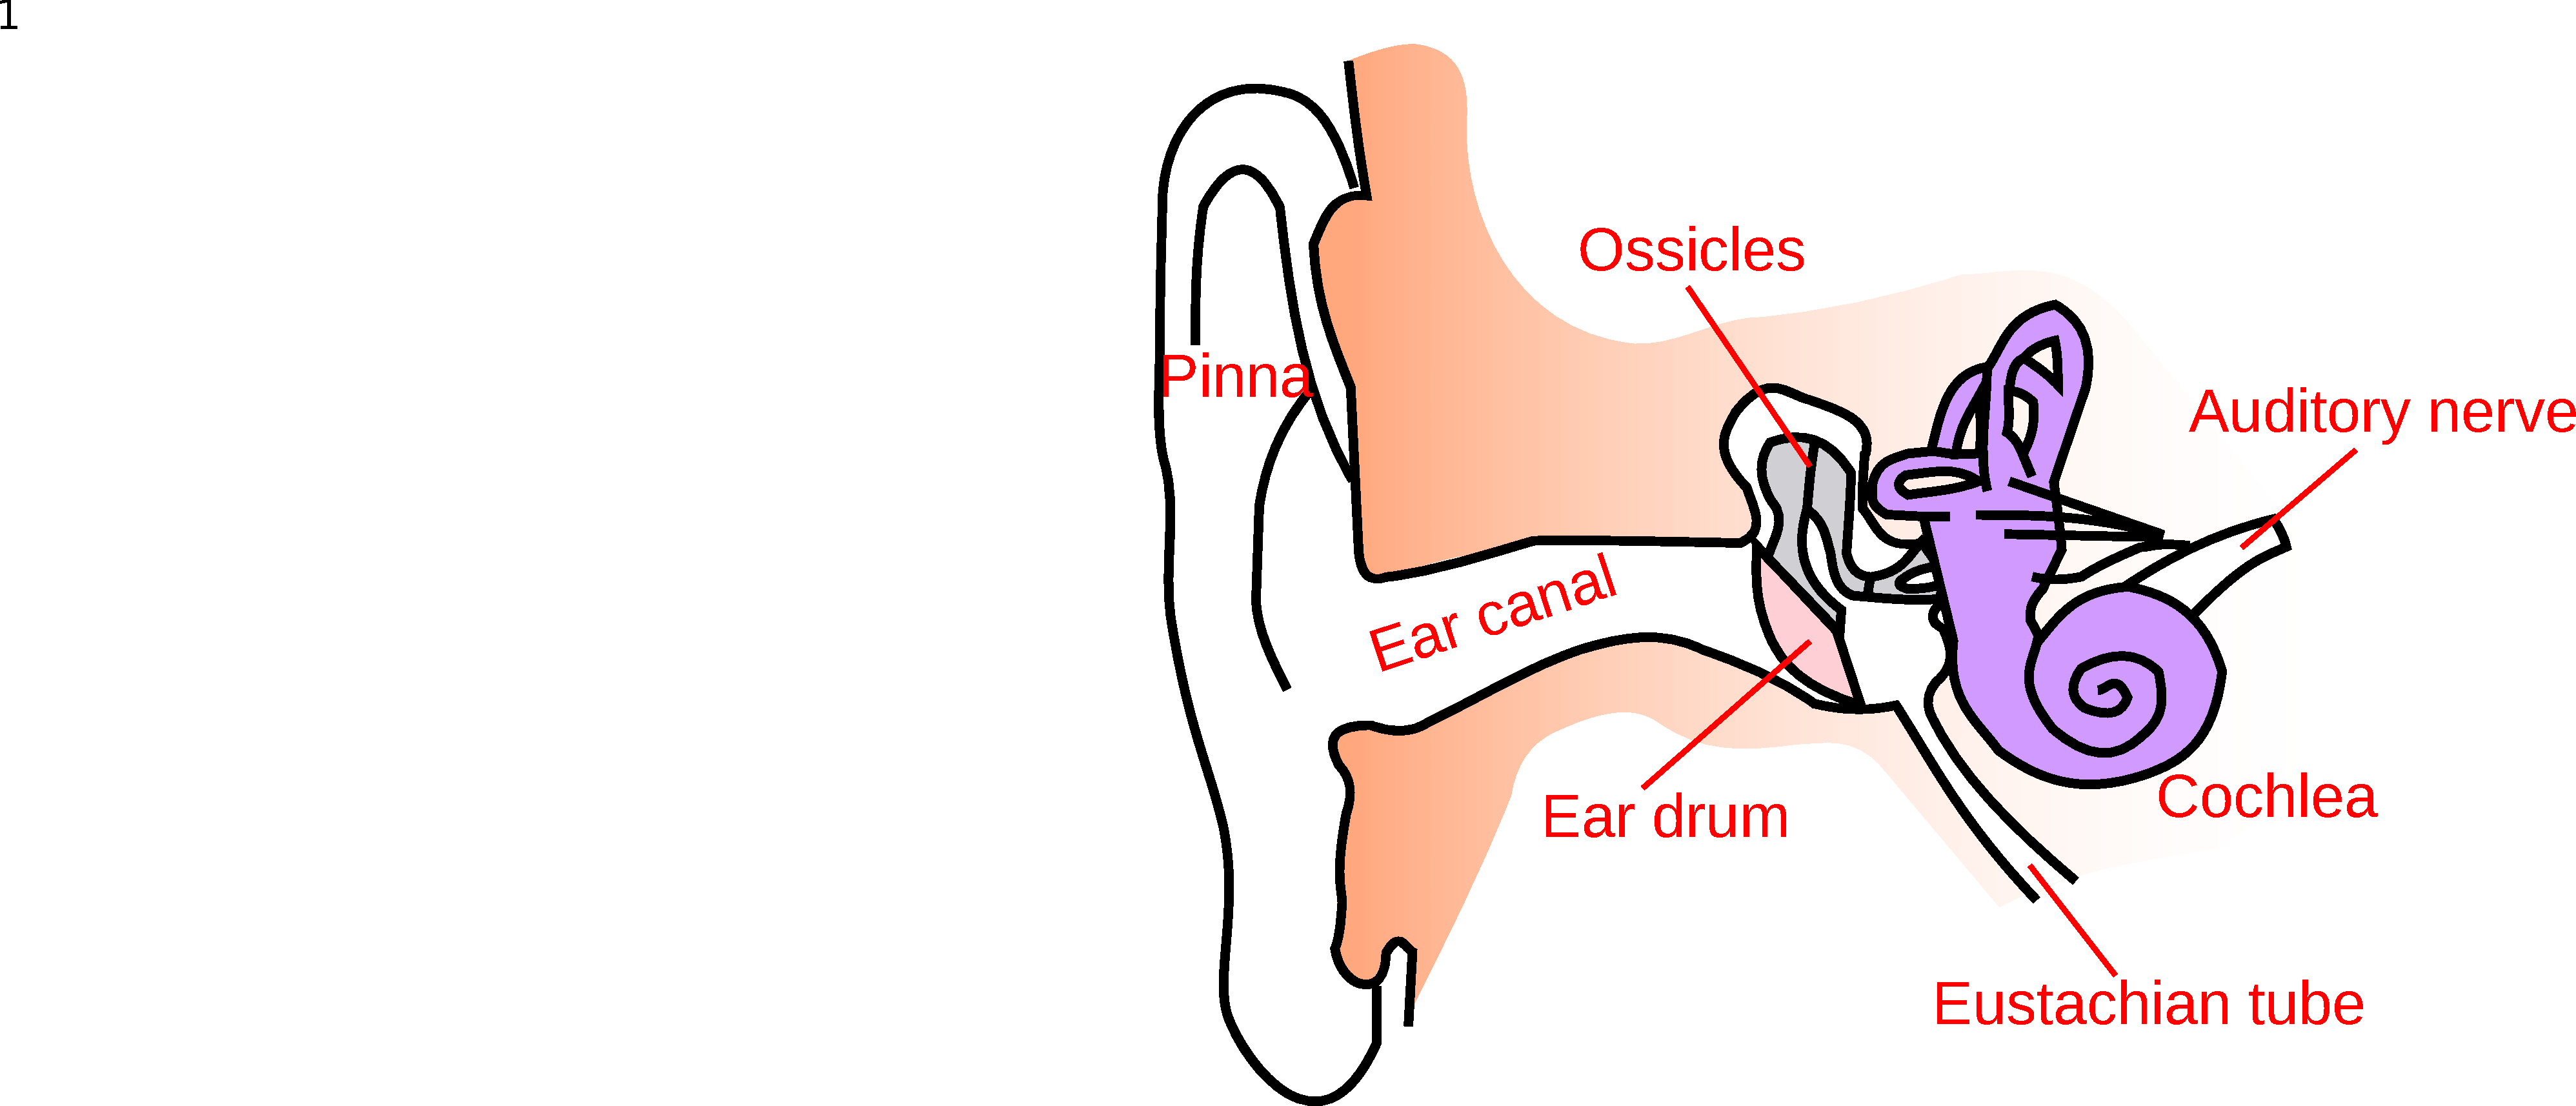
\includegraphics[width=0.7\linewidth]{files/outer-ear-5ba2feb64904b84737321b2ca1e26281.pdf}

\newline
\textit{Image Source: \href{https://en.wikipedia.org/wiki/Outer\_ear}{Wikipedia - Outer Ear}}

The eardrum  in the human ear functions much like the membrane in a microphone. Both act as sensitive barriers that vibrate in response to incoming sound waves. When sound waves enter the ear canal, they strike the eardrum, causing it to vibrate. These vibrations are then transmitted through the ossicles to the inner ear, where they are converted into electrical signals for the brain to interpret. In a microphone, sound waves hit a thin, flexible membrane (diaphragm), causing it to vibrate. These vibrations are converted into electrical signals, which can then be amplified, recorded, or transmitted. As such, both the ear drum and the microphone membrane convert air pressure variations (sound waves) into mechanical vibrations. Both also serve as the first step in transforming acoustic energy into a form that can be further processed; biologically in the ear, electronically in the microphone.

\subsection{The middle ear}

Beyond the eardrum lies the \textit{\href{https://en.wikipedia.org/wiki/Middle\_ear}{middle ear}}, which contains three tiny bones known as the \textit{ossicles}: the malleus, incus, and stapes. These bones act as a mechanical lever system, amplifying the vibrations from the eardrum and transmitting them to the oval window, a membrane-covered opening to the inner ear. This amplification is essential for efficiently transferring sound energy from air to the fluid-filled inner ear.

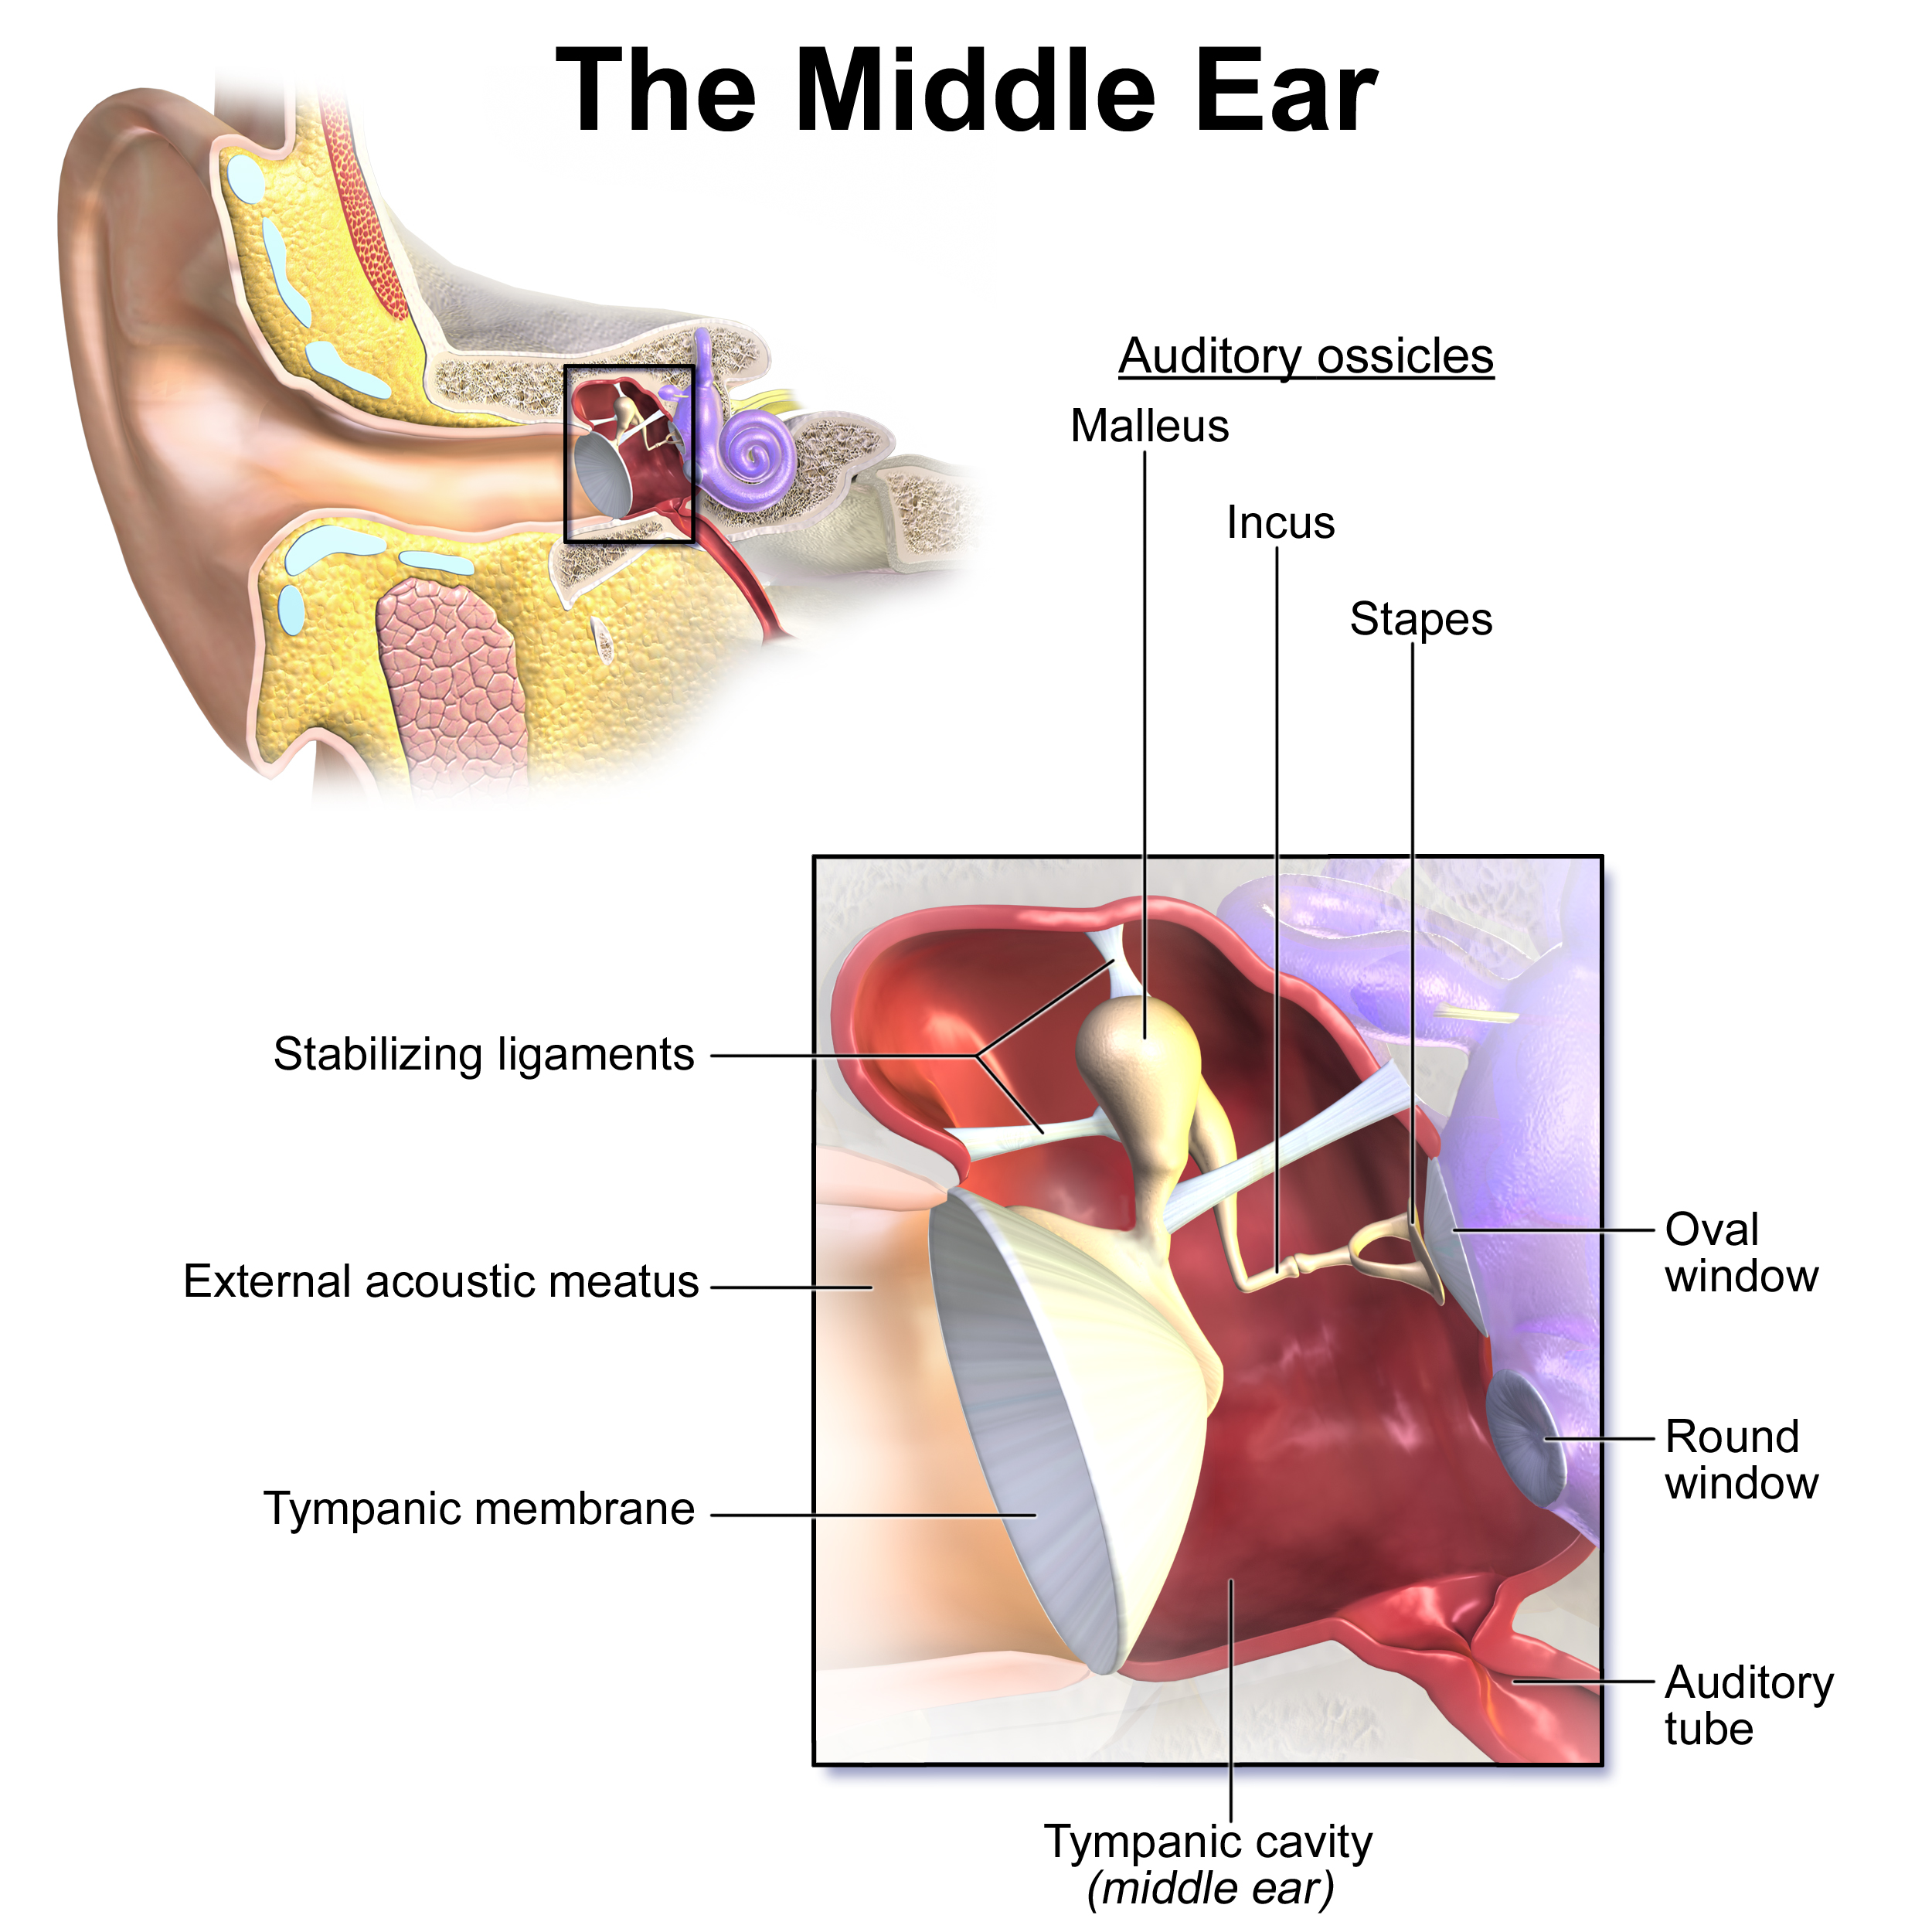
\includegraphics[width=0.7\linewidth]{files/middle-ear-ce6f1838ed24946ab896a19a857929aa.png}

\newline
\textit{Image Source: \href{https://en.wikipedia.org/wiki/Middle\_ear}{Wikipedia - Middle Ear}}

This process is analogous to how a microphone connected to a preamplifier works. The vibrations from a microphone membrane are weak and are typically run through a \textit{preamplifier} to boost the signal to a level suitable for further processing or recording. Similarly, the ossicles amplify the mechanical vibrations from the eardrum, ensuring that the signal is strong enough to be effectively transmitted into the inner ear for further processing by the auditory system.

\subsection{The inner ear}

The \textit{\href{https://en.wikipedia.org/wiki/Inner\_ear}{inner ear}} is where the mechanical vibrations are transformed into electrical signals that the brain can interpret as sound. The main structure responsible for this is the \textit{\href{https://en.wikipedia.org/wiki/Cochlea}{cochlea}}, a spiral-shaped, fluid-filled organ lined with thousands of tiny hair cells. As vibrations travel through the cochlear fluid, they cause the hair cells to move, generating nerve impulses that are sent to the brain via the auditory nerve.

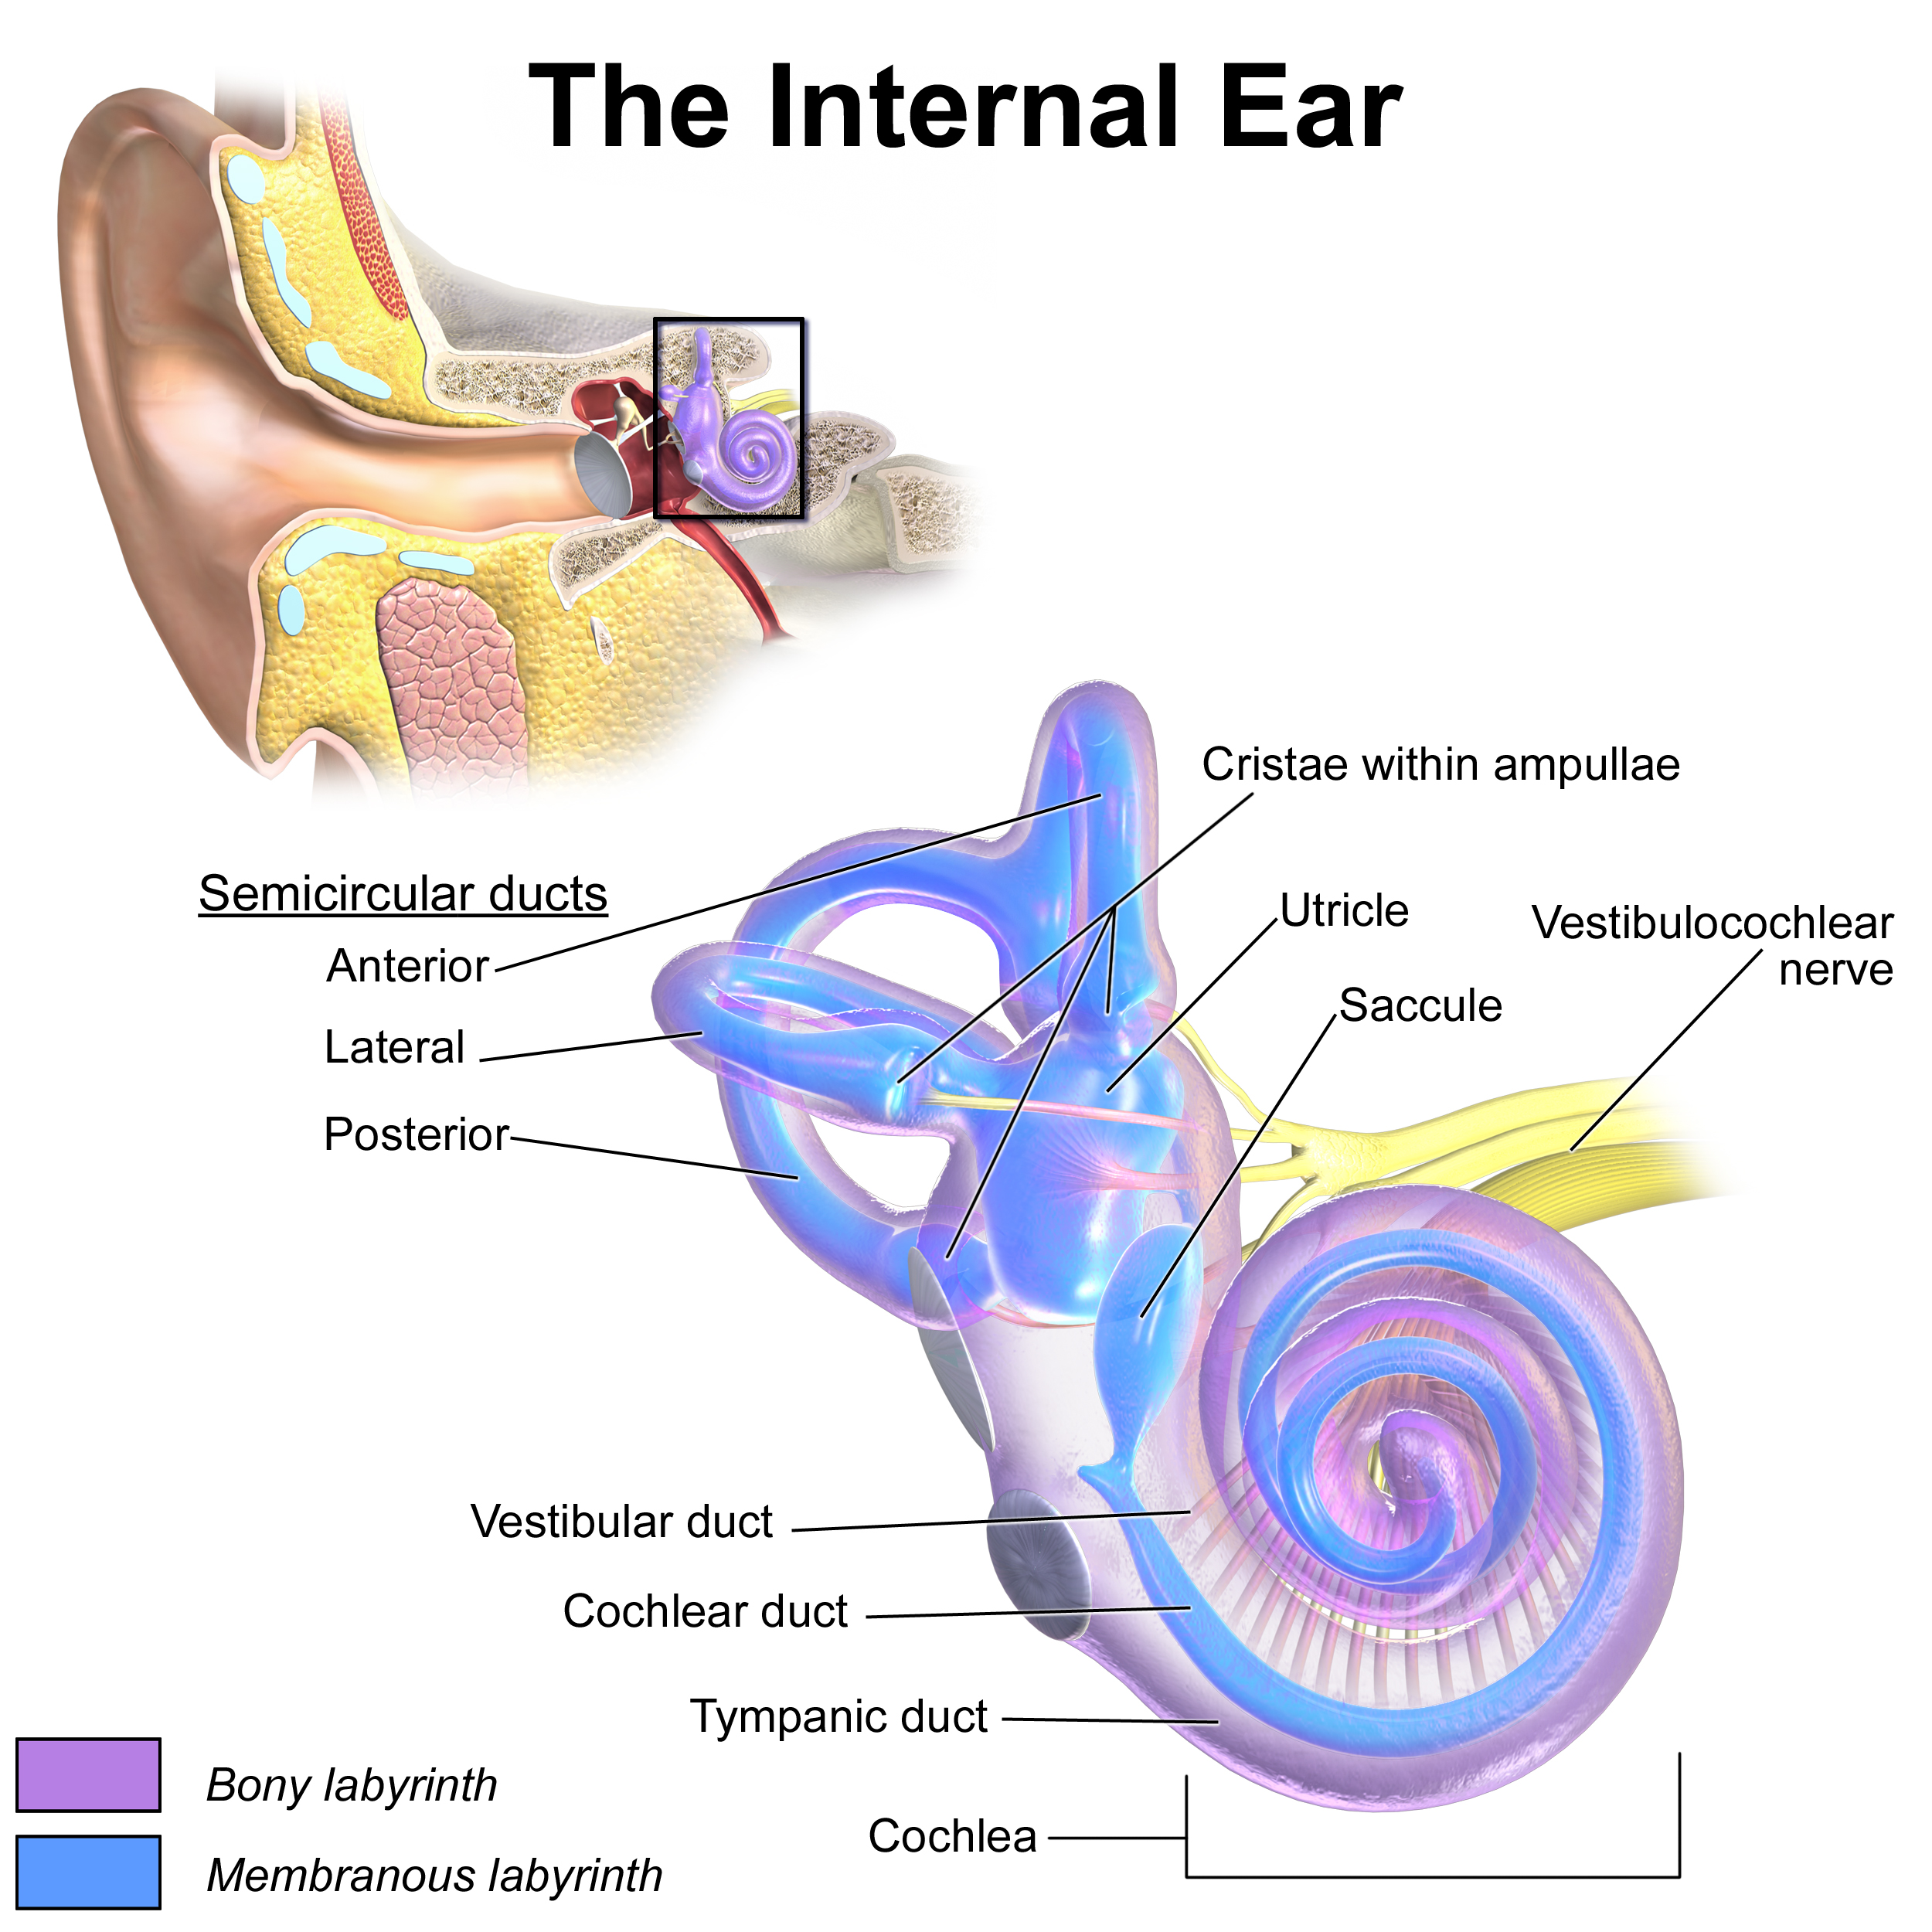
\includegraphics[width=0.7\linewidth]{files/inner-ear-11eec3e05db1f85ae4ead6891a3bbd12.png}

\newline
\textit{Image Source: \href{https://en.wikipedia.org/wiki/Inner\_ear}{Wikipedia - Inner Ear}}

The cochlea in the inner ear functions similarly to an analog-to-digital converter (ADC) in audio technology. Just as an ADC transforms continuous analog sound waves into discrete digital signals that can be processed by computers, the cochlea converts mechanical vibrations from sound into electrical nerve impulses that the brain can interpret. Inside the cochlea, thousands of hair cells respond to specific frequencies, effectively performing a biological form of frequency analysis and encoding the intensity and timing of sounds. This process is analogous to how an ADC samples and quantizes audio signals, enabling the transmission and interpretation of complex auditory information in a form the brain can understand.

The inner ear also contains the \href{https://en.wikipedia.org/wiki/Vestibular\_system}{vestibular system}, which is crucial for maintaining balance and spatial orientation. We will get back to this when we get to music-related body motion.

\subsection{Human vs machine perception}

Although the human auditory system and machine-based audio systems (like microphones and ADCs) are fundamentally different in their biological and technological makeup, drawing analogies between them can help us better understand both. Each system consists of a series of components that transform and process sound, ultimately converting physical vibrations in the air into meaningful information---whether as neural signals in the brain or digital data in a computer.

The different parts are as follows:

\begin{itemize}
\item \textbf{Transduction}: In humans, the ear drum and ossicles convert air pressure variations into mechanical vibrations, while the cochlea transduces these vibrations into electrical nerve impulses. In machines, a microphone membrane converts sound waves into electrical signals, which are then amplified and digitized.
\item \textbf{Frequency Analysis}: The cochlea performs a kind of real-time frequency analysis, with different regions responding to different frequencies (a biological ``filter bank''). Similarly, digital systems use mathematical transforms (like the Fourier Transform) to analyze frequency content.
\item \textbf{Encoding and Transmission}: The auditory nerve encodes and transmits information about sound to the brain, where it is further processed and interpreted. In digital systems, the ADC encodes the analog signal into binary data, which can be stored, transmitted, and processed by computers.
\end{itemize}

Despite these similarities, there are important differences:

\begin{itemize}
\item The human auditory system is adaptive, context-sensitive, and influenced by attention, learning, and memory. It can focus on specific sounds in noisy environments (the ``cocktail party effect'') and fill in missing information based on prior experience.
\item Machine perception is limited by hardware specifications (such as microphone quality and sampling rate) and the algorithms used for analysis. While modern systems can achieve impressive results, they lack the flexibility, nuance, and subjective interpretation of human hearing.
\end{itemize}

Understanding these parallels and differences is essential for fields like audio engineering, hearing aid design, and music information retrieval, where the goal is often to bridge the gap between physical sound and perceptual experience.

\section{Loudness}

If you recall from last week, \textit{\href{https://en.wikipedia.org/wiki/Loudness}{loudness}} is different from \textit{sound pressure level} (SPL). While \textit{\href{https://en.wikipedia.org/wiki/Sound\_pressure\#Sound\_pressure\_level}{sound pressure level (SPL)}} is an objective, physical measurement of the intensity of a sound wave (expressed in decibels, dB), loudness is a subjective perception---how ``loud'' a sound feels to a human listener. Loudness perception is influenced by context, such as background noise and recent exposure to other sounds. This distinction is fundamental in psychoacoustics and underlies many practical considerations in audio engineering, hearing science, and music production.

\subsection{Measuring loudness}

The most common unit for measuring perceived loudness is the \textit{\href{https://en.wikipedia.org/wiki/Phon}{phon}}, which is based on equal-loudness contours (which we will discuss soon). The phon scale is anchored to the loudness of a 1,000 Hz pure tone. For example, a sound that is perceived as equally loud as a 40 dB SPL, 1,000 Hz tone is said to have a loudness of 40 phons, regardless of its frequency or SPL.

There are several standards for estimating loudness in audio signals. \textit{\href{https://en.wikipedia.org/wiki/ITU-R\_BS.1770}{ITU-R BS.1770}} is widely used in broadcasting; this standard defines algorithms for measuring loudness and true-peak audio levels, forming the basis for loudness normalization in radio, TV, and streaming.

Modern audio software and digital audio workstations (DAWs) often include loudness meters that display values in LUFS: \textit{\href{https://en.wikipedia.org/wiki/LUFS}{Loudness units relative to full scale}}. These tools help engineers and producers ensure that audio content meets broadcast standards and provides a comfortable listening experience. When mastering music for streaming platforms, engineers typically aim for an integrated loudness of around -14 LUFS, as recommended by services like Spotify and YouTube. In film and TV, loudness normalization ensures that dialogue, music, and effects are balanced and that viewers do not need to constantly adjust the volume.

\subsection{Threshold of hearing}

The \textit{\href{https://en.wikipedia.org/wiki/Absolute\_threshold\_of\_hearing}{threshold of hearing}} is the quietest sound that the average human ear can detect in a silent environment. This threshold is typically defined as 0 decibels (dB SPL) at 1,000 Hz for a healthy young adult, but it varies with frequency and individual hearing ability. At very low or very high frequencies, sounds must be much louder to be heard.

The threshold of hearing is not a fixed value; it can be affected by age, exposure to loud noises, and even temporary conditions like ear infections or fatigue. As people age, their sensitivity to high frequencies usually decreases, raising the threshold at those frequencies.

The graph below illustrates the average hearing thresholds for different frequencies and age groups, showing how sensitivity changes across the audible spectrum.

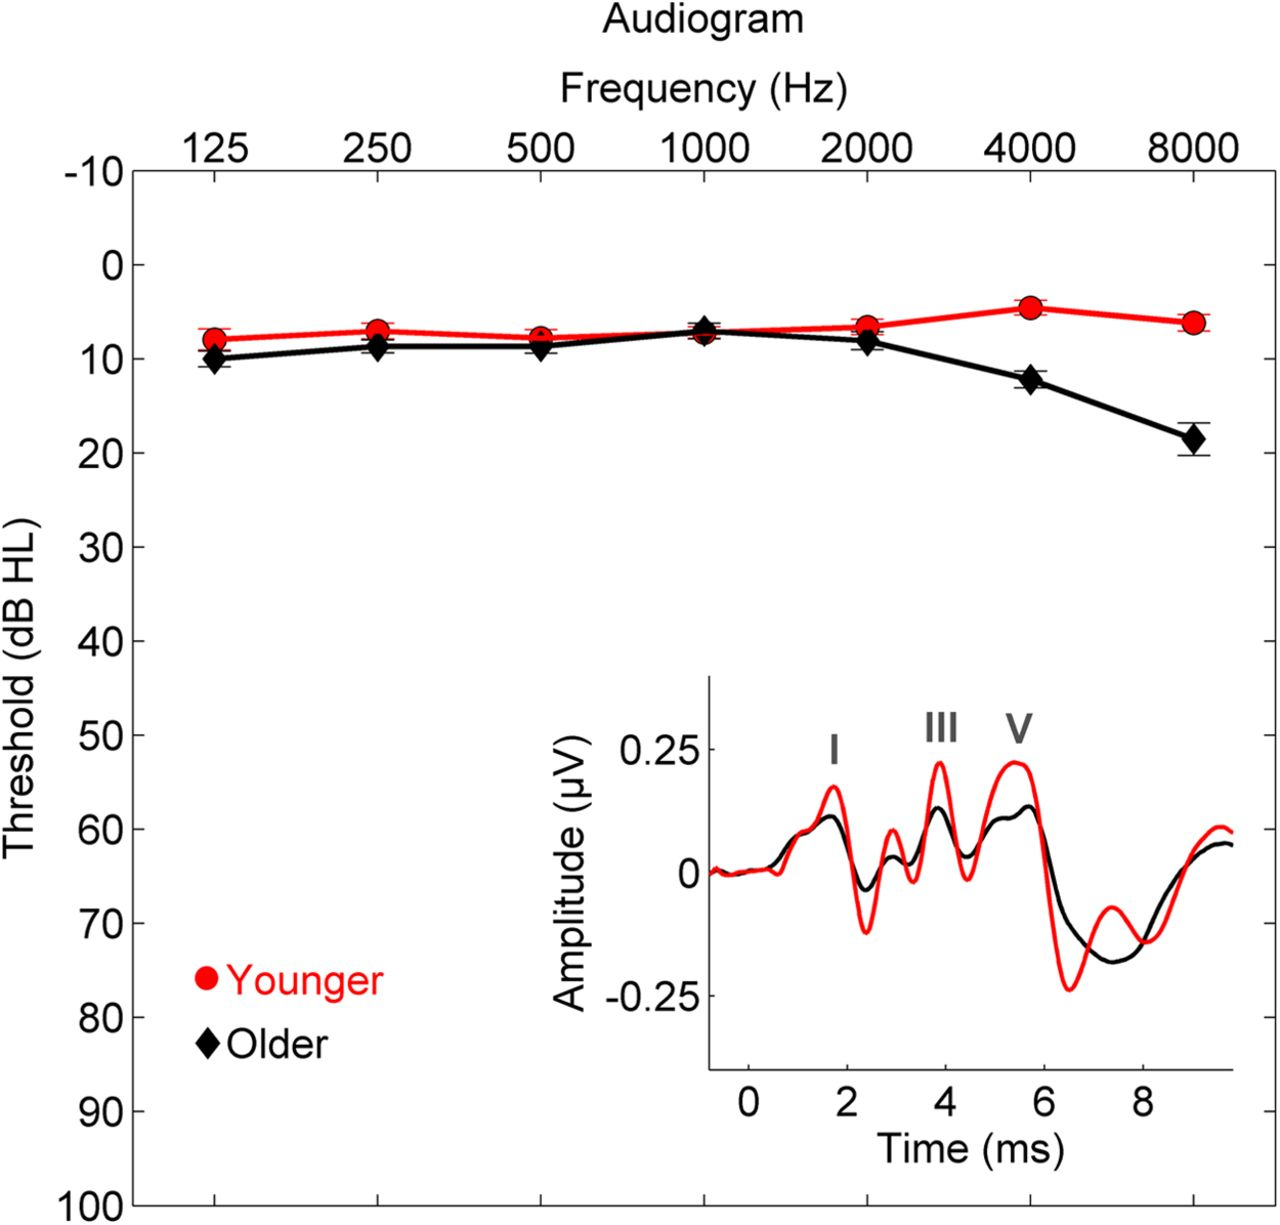
\includegraphics[width=0.7\linewidth]{files/threshold-hearing-bcb5f5f25ba608e2ff8358c8a0f61b31.jpg}


\textit{Image Source: \href{https://en.wikipedia.org/wiki/Absolute\_threshold\_of\_hearing}{Wikipedia - Hearing Thresholds}}

\subsection{Safe listening levels}

Here is a list of some different sound levels:

\bigskip\noindent
\begin{tabular}{p{\dimexpr 0.333\linewidth-2\tabcolsep}p{\dimexpr 0.333\linewidth-2\tabcolsep}p{\dimexpr 0.333\linewidth-2\tabcolsep}}
\toprule
Sound Source & Approximate Loudness (dB SPL) & Example / Context \\
\hline
Threshold of hearing & 0 & Quietest sound a healthy ear can detect \\
Rustling leaves & 10 & Very quiet, barely audible \\
Whisper & 20--30 & Soft whisper at close distance \\
Quiet library & 30--40 & Typical background noise \\
Normal conversation & 60 & At 1 meter distance \\
Busy street traffic & 70--85 & Inside a car with windows closed \\
Subway train & 95--100 & Inside the train \\
Rock concert & 110--120 & Near speakers \\
Threshold of pain & 130 & Jet engine at 30 meters \\
Fireworks / Gunshot & 140--150 & Close range \\
\bottomrule
\end{tabular}

\bigskipAs a rule of thumb, prolonged exposure to sounds above 85 dB can cause hearing damage. For example, typical conversation is around 60 dB, city traffic can reach 85 dB, and concerts or clubs often exceed 100 dB. The higher the volume, the shorter the safe exposure time. At 100 dB, hearing damage can occur in as little as 15 minutes.

The World Health Organization (WHO) recommends keeping personal listening devices below 80 dB for adults (75 dB for children) and limiting exposure to loud environments. Using ear protection in noisy settings and taking listening breaks can help preserve hearing health.

Sounds above 120--130 dB (such as jet engines at close range or fireworks) can cause immediate pain and permanent hearing loss. Even brief exposure to extremely loud sounds can result in irreversible damage to the hair cells in the inner ear.

\begin{framed}
\textbf{Question}\\
How do you protect your hearing?
\end{framed}

\subsection{Equal Loudness Contours}

One important thing to consider is that there is not a direct relationship between \href{https://en.wikipedia.org/wiki/Sound\_pressure\#Sound\_pressure\_level}{sound pressure level (SPL)} and \href{https://en.wikipedia.org/wiki/Loudness}{loudness}. Although they are related, the same SPL can be perceived as having a different loudness depending on the frequency of the sound and the listener's hearing sensitivity.

This relationship was first systematically studied by \href{https://en.wikipedia.org/wiki/Harvey\_Fletcher}{Harvey Fletcher} and \href{https://en.wikipedia.org/wiki/Wilden\_A.\_Munson}{Wilden A. Munson} in the 1930s. Their experiments led to the creation of the \textit{Fletcher-Munson curves}, which is nowadays often also known as \textit{\href{https://en.wikipedia.org/wiki/Equal-loudness\_contour}{equal-loudness contours}}. These curves show that the human ear is not equally sensitive to all frequencies: we are most sensitive to frequencies between roughly 2,000 and 5,000 Hz, and less sensitive to very low or very high frequencies. As a result, a low-frequency sound must be played at a higher SPL than a mid-frequency sound to be perceived as equally loud.

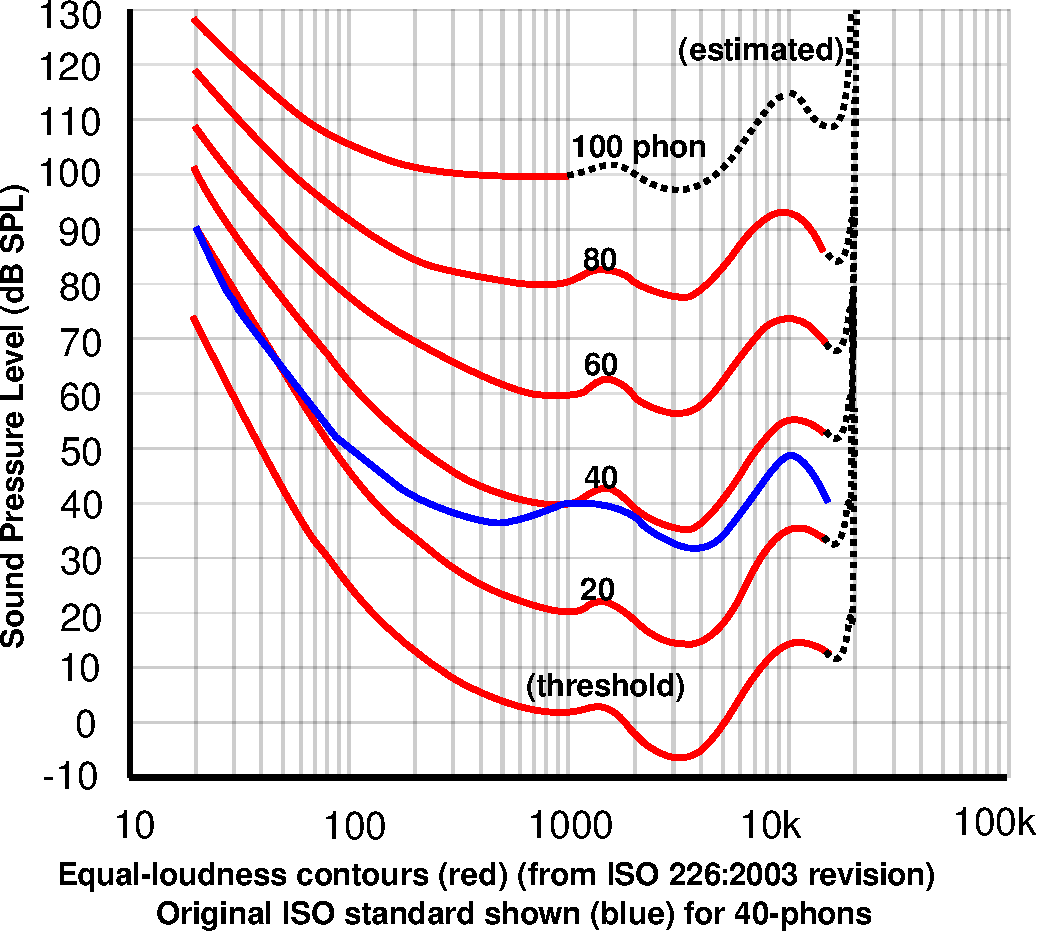
\includegraphics[width=0.7\linewidth]{files/equal-loudness-d4c86bb8aa88310a08b6040a7286beb8.pdf}


\textit{Image Source: \href{https://en.wikipedia.org/wiki/Equal-loudness\_contour}{Wikipedia - Equal-loudness contour}}

There is evidence suggesting that our heightened sensitivity to frequencies between 2,000 and 5,000 Hz has evolutionary roots. This frequency range corresponds closely to the spectral content of human speech, particularly the consonant sounds that are crucial for understanding language. Being able to detect subtle differences in these frequencies would have provided a survival advantage by improving communication, social bonding, and the ability to detect important environmental sounds such as a baby's cry or warning calls. Over time, natural selection may have favored individuals whose hearing was optimized for these frequencies, shaping the contours of human auditory perception.

Equal-loudness contours are crucial in audio engineering, music production, and hearing science. They explain why music or speech can sound different at low versus high volumes, and why audio equipment often includes ``loudness'' compensation to adjust for these perceptual differences. Understanding these contours helps us design better audio systems and create more accurate sound reproductions that align with human hearing.

\subsection{Just noticeable differences for loudness}

The \textit{\href{https://en.wikipedia.org/wiki/Just-noticeable\_difference}{just noticeable difference}} (JND), also called the \textit{difference limen}, is the smallest change in a physical stimulus that a listener can reliably detect. For loudness, the JND refers to the smallest change in sound intensity that can be perceived as a difference in loudness by a human listener.

The JND for loudness is often expressed as a percentage of the original sound level. For mid-level sounds, the JND is typically about 1 dB (decibel), meaning that a change of at least 1 dB is needed for most people to notice a difference in loudness. This threshold can vary depending on the frequency, the absolute loudness, and the listening environment.

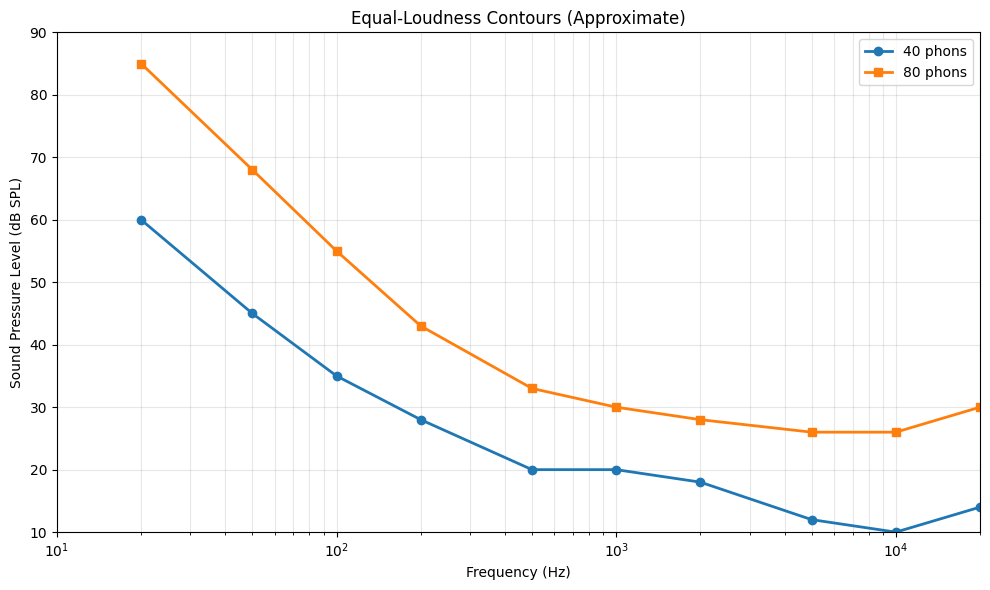
\includegraphics[width=0.7\linewidth]{files/9084cdb7c12be1261e4632ea827c6645.png}

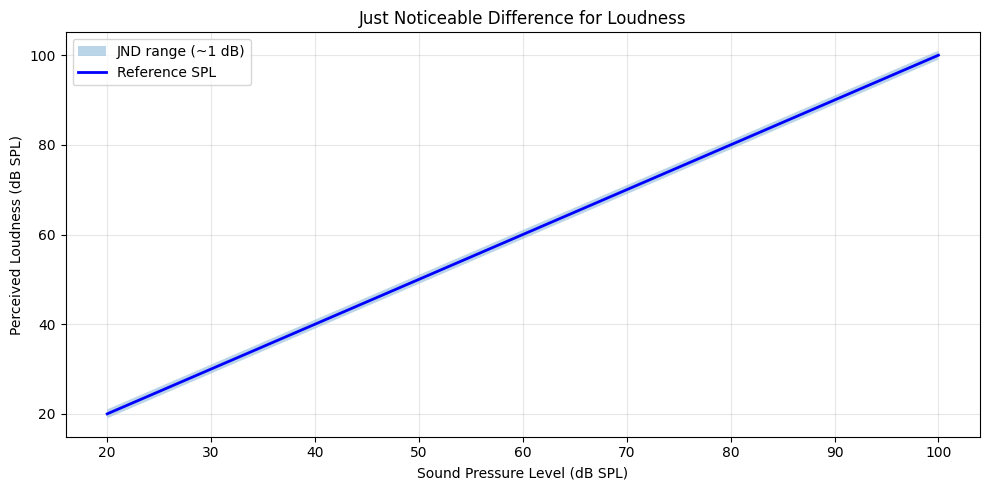
\includegraphics[width=0.7\linewidth]{files/681dfb7151d790f944b1505cd5db4c78.png}

\section{Pitch}

When we hear tonal sounds, like musical instruments but also voices, we typically hear a \textit{pitch}. The pitch is closely related to the physical property of frequency (the rate at which a sound wave vibrates), but it is ultimately a subjective experience shaped by the human auditory system.

\subsection{Pitch range}

The typical range of audible sound for humans spans from approximately \href{https://en.wikipedia.org/wiki/Hertz}{20 Hz} to \href{https://en.wikipedia.org/wiki/Hearing\_range}{20,000 Hz}, encompassing the frequencies we perceive as \href{https://en.wikipedia.org/wiki/Pitch\_(music)}{pitch}. Sounds below 20 Hz are referred to as \href{https://en.wikipedia.org/wiki/Infrasound}{infrasound} and are generally imperceptible to the human ear, while those above 20,000 Hz are called \href{https://en.wikipedia.org/wiki/Ultrasound}{ultrasound} and also lie beyond our hearing range. Within the audible spectrum, our sensitivity to pitch and frequency varies, with the greatest acuity in the mid-frequency range, which is crucial for understanding speech and music.

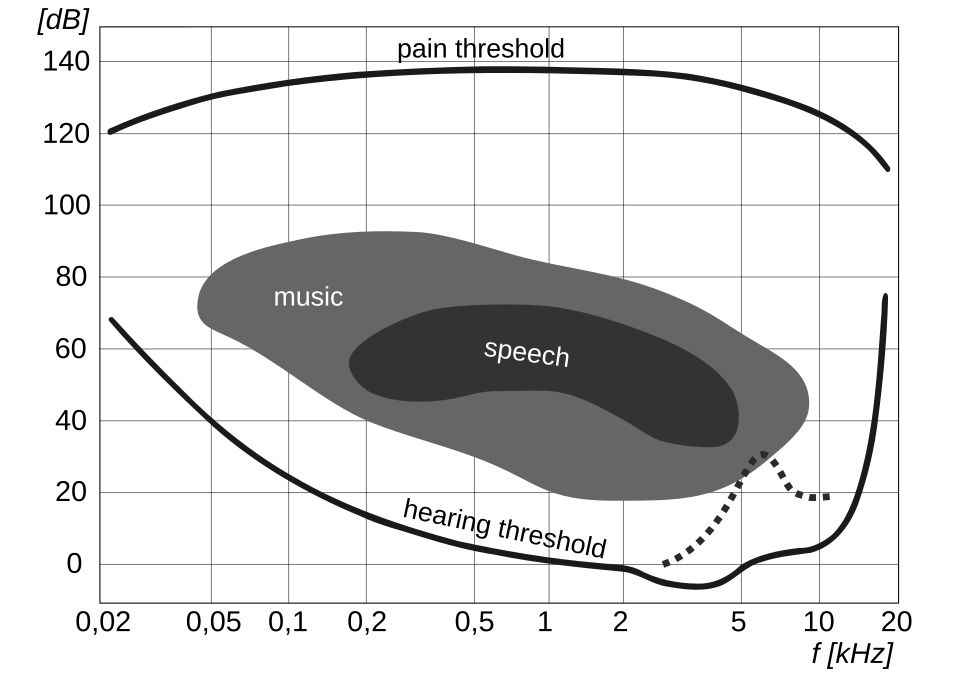
\includegraphics[width=0.7\linewidth]{files/human-hearing-639bcd1dc535e45b0021a45a73c5856c.png}

It is well-known that dogs have better hearing than humans, and the following graphs show that humans are in the middle of the pitch range among animals. Different animal species have evolved to detect sounds in frequency ranges that are most relevant to their survival and communication. For example, dogs can hear frequencies up to around 45,000 Hz, allowing them to detect high-pitched noises that are inaudible to humans. Bats and dolphins can perceive even higher frequencies, well into the ultrasonic range, which they use for echolocation. On the other hand, elephants and some whales can hear infrasound---very low frequencies below the human hearing threshold---which helps them communicate over long distances.

The chart below compares the hearing ranges of various animals, illustrating how human hearing fits within the broader spectrum of animal auditory perception. This diversity in hearing abilities reflects the different ecological needs and evolutionary pressures faced by each species. Understanding these differences not only highlights the uniqueness of human hearing but also provides insight into how other animals experience the world of sound.

\includegraphics[width=0.7\linewidth]{files/animal-hearing-5a3f71492cc6bae0cb471bde7cedb094.pdf}

\subsection{Just Noticeable Differences for pitch}

We have a just noticeable difference (JND) also for pitch, which relates to the smallest change in frequency that a listener can reliably detect. The human ear is highly sensitive to small frequency changes, especially in the mid-frequency range (about 500--4000 Hz, where speech and music are most prominent). For example, at 1000 Hz, the JND for pitch is typically around 3 Hz for trained listeners, which is about 0.3\% of the frequency. This means that if you play two tones at 1000 Hz and 1003 Hz, a trained listener can usually tell them apart. At very low or very high frequencies, the JND becomes larger, meaning it is harder to distinguish small pitch differences.

The JND for pitch vary depending on factors such as the listener's age, hearing ability, training, the loudness of the tones, and whether the tones are played in isolation or in a complex sound environment.

\section{Timbre}

\textit{\href{https://en.wikipedia.org/wiki/Timbre}{Timbre}} is the quality of a sound that distinguishes different types of sound sources, even when they have the same pitch and loudness. It is what allows us to tell apart a piano and a violin playing the same note at the same volume. Timbre is shaped by the spectral content (the mix of the \textit{fundamental} and the \textit{overtones}), the temporal envelope (attack, decay, sustain, release), and other characteristics such as vibrato or noise components. In music and audio, timbre is essential for identifying instruments, voices, and sound textures.

\subsection{Overtones}

When a musical instrument or voice produces a note, it doesn't just generate a single frequency (the \textit{fundamental}), but also a series of higher frequencies called \textit{overtones} or \textit{harmonics}. These overtones are integer multiples of the fundamental frequency and contribute to the richness and color of the sound.

\begin{itemize}
\item \textbf{Fundamental}: The lowest frequency of a sound, typically perceived as its pitch.
\item \textbf{Overtones/Harmonics}: Frequencies above the fundamental. The first overtone is the second harmonic (2$\times$ the fundamental), the second overtone is the third harmonic (3$\times$ the fundamental), and so on.
\end{itemize}

A pure sine wave has no overtones and sounds ``plain'' or ``pure,'' while most musical sounds are complex and rich due to their overtone content. The specific pattern and strength of overtones determine the timbre of an instrument. For example, a clarinet and a violin playing the same note will have different overtone structures, making them sound distinct.

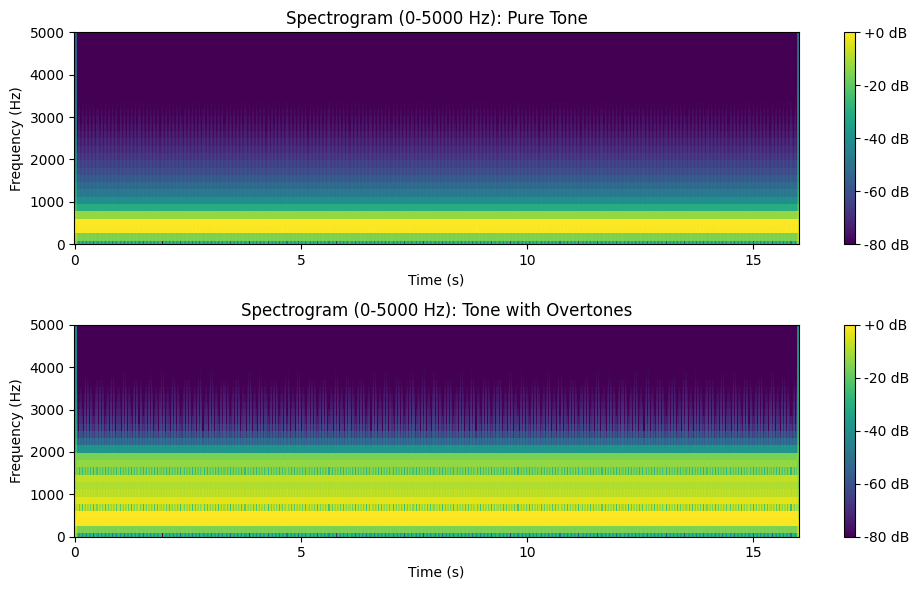
\includegraphics[width=0.7\linewidth]{files/d8fd1fc8bf2dec2ef2d56eab6b1b5dea.png}

\subsection{Envelope}

The \textit{\href{https://en.wikipedia.org/wiki/Envelope\_(waves)}{envelope}} of a sound describes how its amplitude changes over time, shaping the sound's overall character and dynamics. The envelope determines how a sound starts, develops, and ends, and is crucial for distinguishing between different instruments and sound types.

In audio synthesis, the most common model is the \textit{\href{https://en.wikipedia.org/wiki/Synthesizer\#ADSR\_envelope}{ADSR envelope}}, which stands for \textbf{Attack}, \textbf{Decay}, \textbf{Sustain}, and \textbf{Release}:

\begin{itemize}
\item \textbf{Attack}: The time it takes for the sound to reach its maximum amplitude after being triggered.
\item \textbf{Decay}: The time it takes for the amplitude to decrease from the peak level to the sustain level.
\item \textbf{Sustain}: The level at which the sound holds while the note is sustained.
\item \textbf{Release}: The time it takes for the sound to fade to silence after the note is released.
\end{itemize}

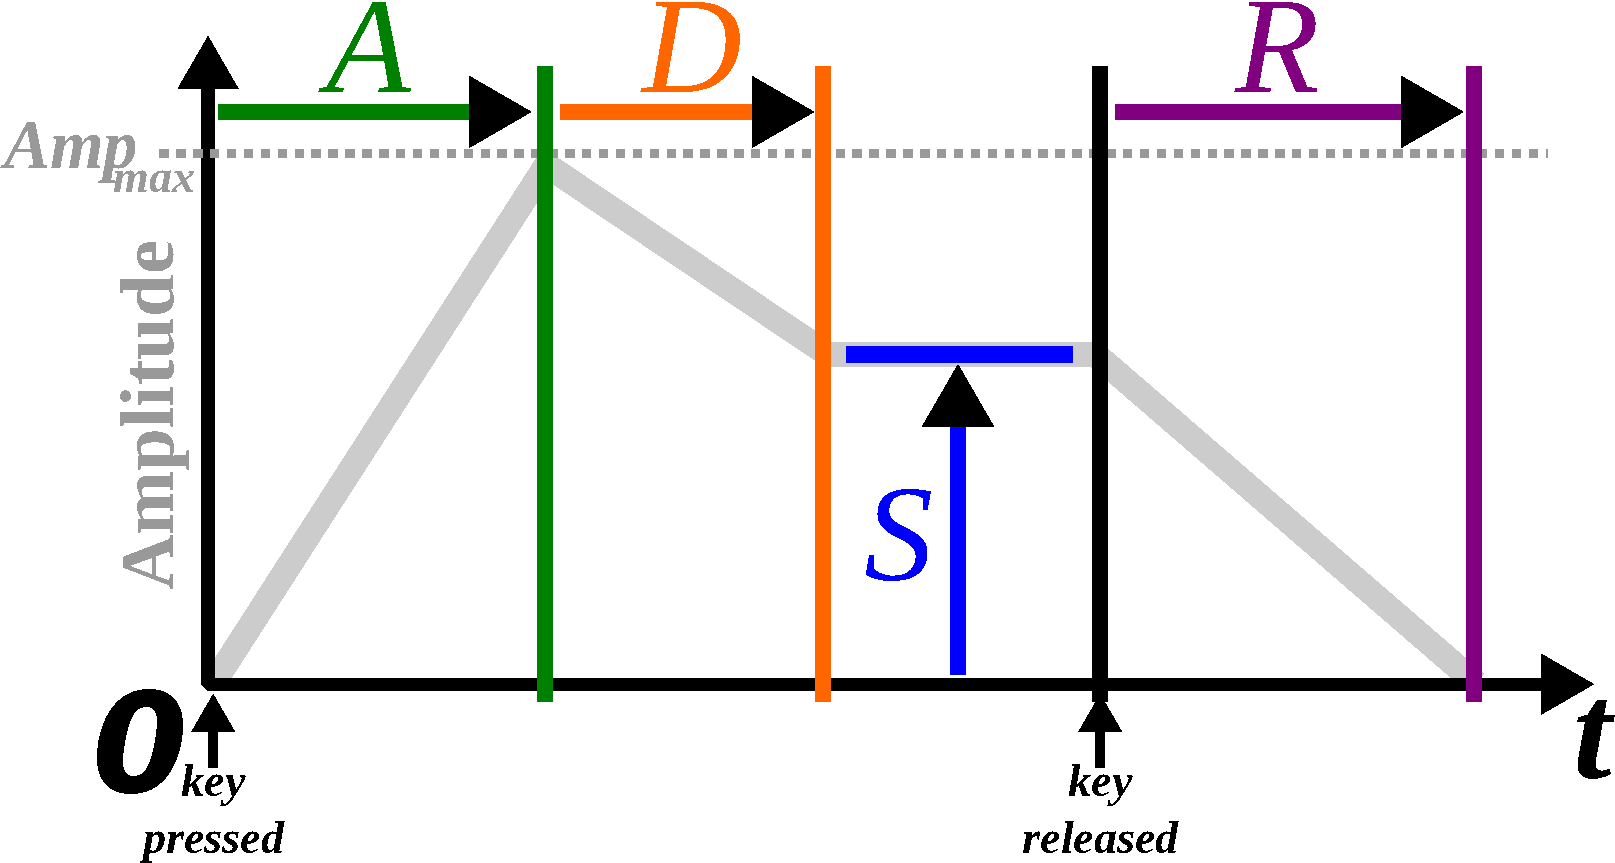
\includegraphics[width=0.7\linewidth]{files/adsr-0f73521fb430eba6818a89bab07f1507.pdf}


\textit{Image source: \href{https://en.wikipedia.org/wiki/Synthesizer\#ADSR\_envelope}{ADSR envelope on Wikipedia}.}

\subsection{Just noticeable differences of timbre}

How many partials do you need to recognize the timbre of a sound. Below you can find examples of a Sony Rollins saxophone tone that has been spectrally decomposed and with resynthesis of an increasing number of overtones.

\begin{verbatim}
Found 0 audio files:
\end{verbatim}

\section{Spatial perception}

\textit{\href{https://en.wikipedia.org/wiki/Sound\_localization}{Spatial hearing}} refers to our ability to perceive the location and movement of sound sources in our environment. This skill allows us to determine where a sound is coming from---whether it is in front, behind, above, below, or to the side. Spatial hearing is essential for navigating the world, understanding speech in complex environments, and enjoying immersive audio experiences in music and virtual reality.

\href{https://en.wikipedia.org/wiki/Binaural\_hearing}{Binaural hearing} is the process of using both ears to perceive spatial cues and localize sounds. By comparing the differences in timing (ITD) and intensity (ILD) between the two ears, the brain constructs a three-dimensional auditory scene. Binaural hearing is essential for depth perception, sound localization, and separating different sound sources in complex environments.

\subsection{Interaural time difference}

The \href{https://en.wikipedia.org/wiki/Sound\_localization\#Interaural\_time\_difference}{interaural time difference (ITD)} is the difference in the arrival time of a sound at each ear. When a sound source is positioned off-center, it reaches one ear slightly before the other. The brain uses this tiny time difference, especially for low-frequency sounds, to help localize the direction of the sound source on the horizontal plane. ITD is a primary cue for determining the azimuth (left-right position) of sounds.

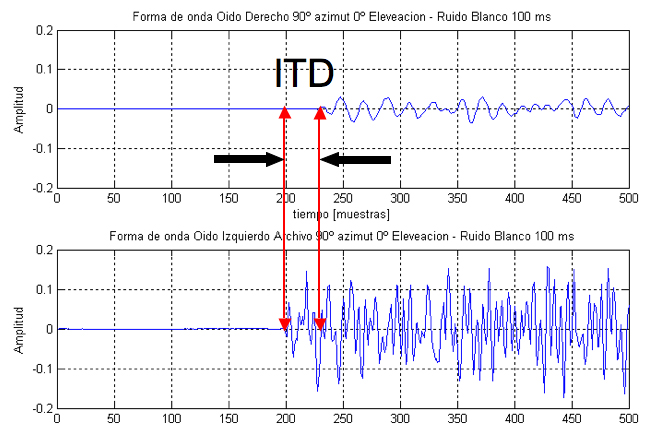
\includegraphics[width=0.7\linewidth]{files/itd-f0cfc03b564b6637ffe3fc76f47dbd38.jpg}

\subsection{Interaural level difference}

\href{https://en.wikipedia.org/wiki/Sound\_localization\#Interaural\_level\_difference}{Interaural level difference (ILD)} refers to the difference in sound pressure level reaching each ear. When a sound comes from one side, the head acts as a barrier, causing the sound to be louder in the ear closer to the source and quieter in the far ear. ILD is most effective for high-frequency sounds, where the head shadow effect is more pronounced. The brain combines ILD with ITD to accurately localize sounds.

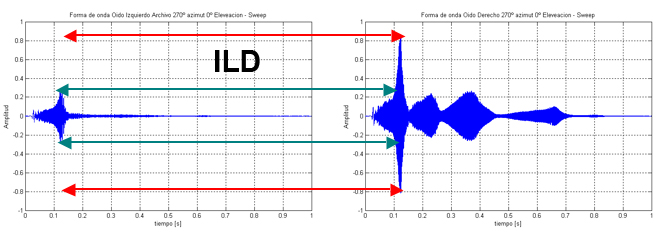
\includegraphics[width=0.7\linewidth]{files/ild-ff508efb9641c988dedeb70bbf761c42.jpg}

\subsection{Head-related transfer function}

The \href{https://en.wikipedia.org/wiki/Head-related\_transfer\_function}{head-related transfer function (HRTF)} describes how an ear receives a sound from a specific point in space, taking into account the effects of the listener's head, torso, and outer ear (pinna). HRTFs are unique to each individual and are crucial for perceiving elevation and front-back differences in sound localization. They are widely used in 3D audio and virtual reality to simulate realistic spatial audio experiences.

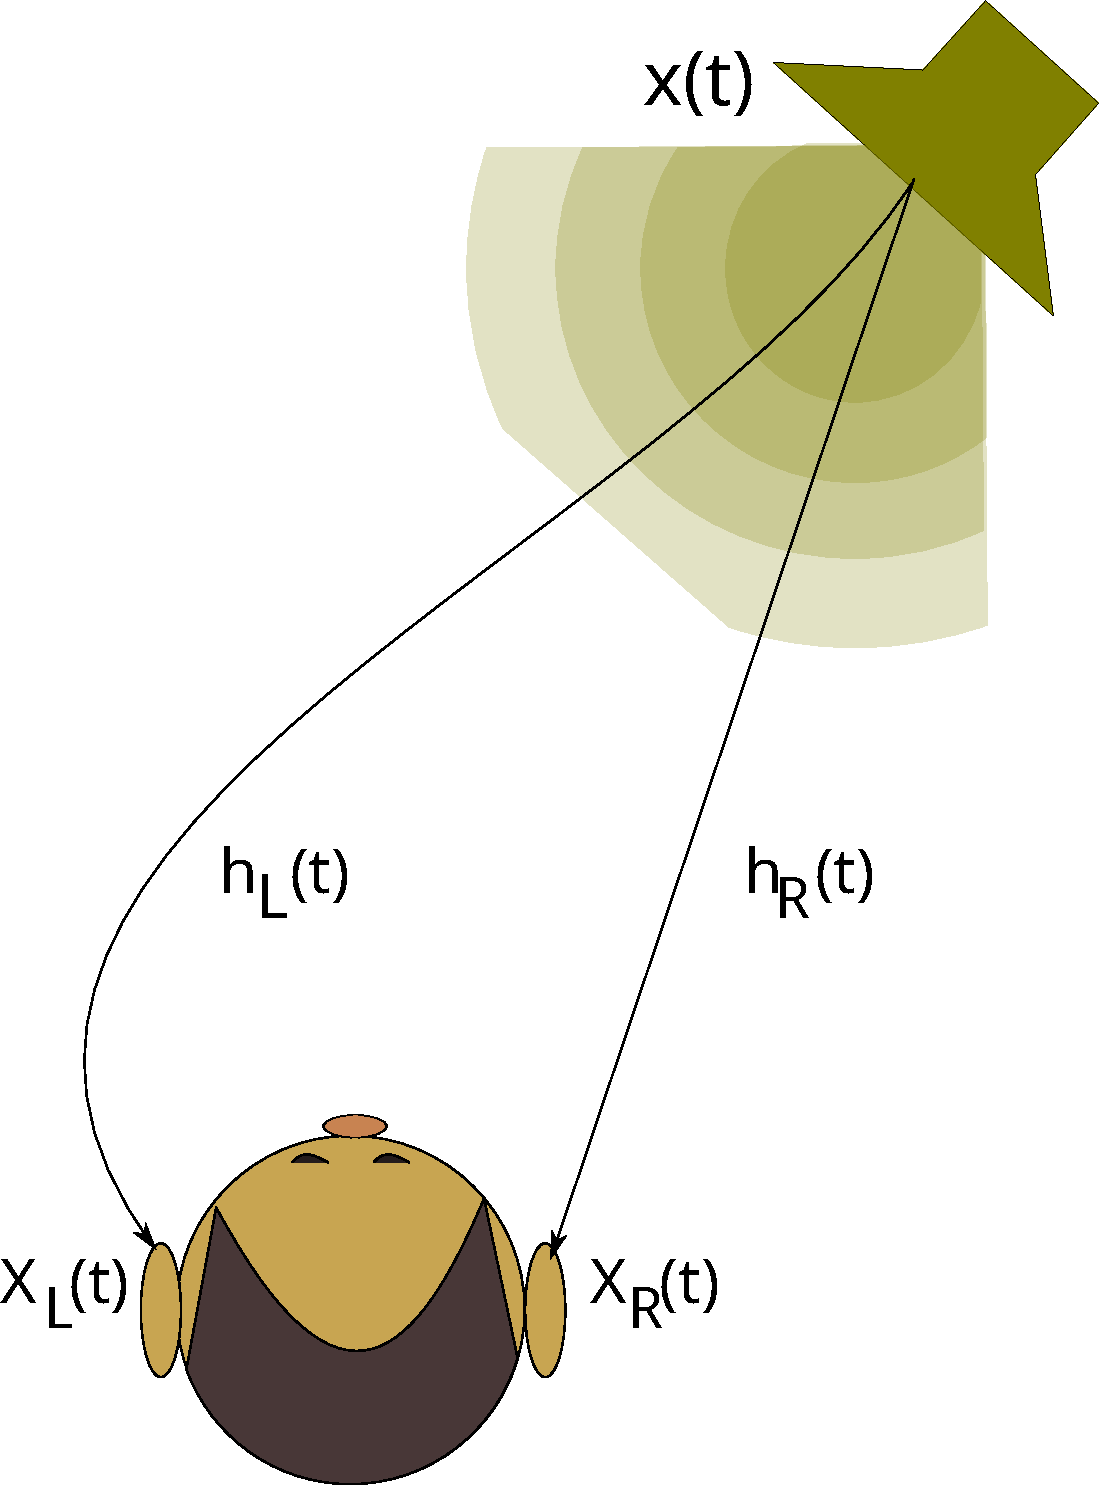
\includegraphics[width=0.7\linewidth]{files/hrtf-83fb3886a713cc817ff236fde085b241.pdf}

The \href{https://en.wikipedia.org/wiki/Precedence\_effect}{precedence effect} is a phenomenon where the first-arriving sound dominates our perception of the sound's location, even if reflections or echoes follow shortly after. This effect helps us focus on the direct sound source in reverberant environments, such as distinguishing a speaker's voice in a large hall, and prevents confusion from multiple sound reflections.

\subsection{Cocktail party effect}

The \href{https://en.wikipedia.org/wiki/Cocktail\_party\_effect}{cocktail party effect} describes our remarkable ability to focus on a single sound source, such as a conversation partner, in a noisy environment filled with competing sounds. This selective attention relies on spatial hearing cues, as well as cognitive processes, to filter out background noise and enhance the target sound. The cocktail party effect is a key aspect of auditory scene analysis and is fundamental to effective communication in social settings.

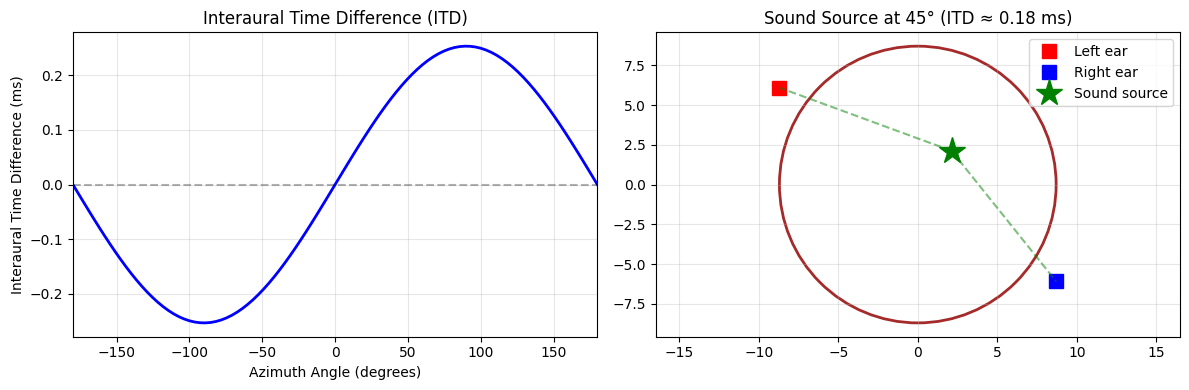
\includegraphics[width=0.7\linewidth]{files/ecf80e6d4f0e33b7ca01adbf3a8552c1.png}

\section{Auditory illusions}

Auditory illusions are fascinating because they reveal the complex ways in which our brains interpret sound, often going beyond the raw physical properties of audio signals. By studying these illusions, we gain insight into the mechanisms of human auditory perception, how we organize, prioritize, and sometimes misinterpret acoustic information. This understanding is crucial for fields like music production, audio engineering, hearing aid design, and the development of perceptually efficient audio codecs.

\subsection{Hysteresis}

\textit{\href{https://en.wikipedia.org/wiki/Hysteresis}{Hysteresis}} refers to the phenomenon where the response of a system depends not only on its current state but also on its past states. In psychoacoustics, hysteresis can be observed in loudness perception: the perceived loudness of a sound may depend on the sequence of sounds that came before it. For example, if a listener is exposed to a loud sound and then to a softer sound, the softer sound may seem even quieter than if it were heard in isolation. Conversely, a gradual increase in volume may be perceived differently than a sudden jump, even if the final sound pressure level is the same. This effect highlights how our auditory system adapts to changing sound environments and why context and listening history can influence how loud a sound seems.

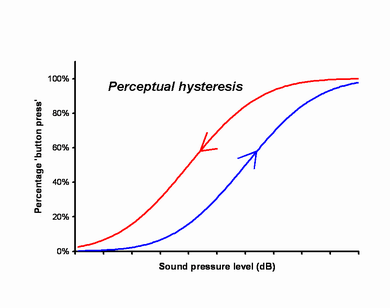
\includegraphics[width=0.7\linewidth]{files/hysteresis-4090fefebb34628ecd8154ac838cfcd8.png}


\textit{Image Source: \href{https://en.wikipedia.org/wiki/Hysteresis}{Wikipedia - Hysteresis}}

\subsection{Masking Effects}

\textit{Masking} in psychoacoustics refers to the phenomenon where the presence of one sound (the masker) makes it more difficult to hear another sound (the maskee). This occurs because the auditory system has limited frequency and temporal resolution, so strong or similar sounds can ``cover up'' weaker or nearby sounds, making them less perceptible or even inaudible.

There are different types of masking. \href{https://en.wikipedia.org/wiki/Masking\_(psychophysics)\#Simultaneous\_masking}{Simultaneous Masking} refers to when two sounds are played at the same time, a louder sound (the masker) can make a softer sound (the maskee) inaudible, even if both are within the listener's hearing range. This effect is strongest when the sounds are close in frequency. For example, in music production, a loud bass drum can mask a softer bass guitar note if they occur together and share similar frequencies. This principle is used in \href{https://en.wikipedia.org/wiki/Audio\_compression\_(data)}{audio compression}, such as \href{https://en.wikipedia.org/wiki/MP3}{MP3}, which remove masked sounds to reduce file size without noticeably affecting perceived audio quality.

\href{https://en.wikipedia.org/wiki/Masking\_(psychophysics)\#Frequency\_masking}{Frequency Masking} is most effective when the masker and maskee are close in frequency, typically within the same \href{https://en.wikipedia.org/wiki/Critical\_band}{critical band}. The human ear divides the frequency spectrum into critical bands, and sounds within the same band are more likely to mask each other. This is why a high-pitched sound is less likely to be masked by a low-pitched sound, and vice versa. Masking is generally stronger for frequencies above the masker (upward spread) than for those below. This means a loud low-frequency sound can mask higher-frequency sounds more effectively than the reverse.

\href{https://en.wikipedia.org/wiki/Masking\_(psychophysics)\#Temporal\_masking}{Temporal Masking} refers to when a loud sound can mask a softer sound that occurs immediately before (\href{https://en.wikipedia.org/wiki/Masking\_(psychophysics)\#Pre-masking}{pre-masking}) or after (\href{https://en.wikipedia.org/wiki/Masking\_(psychophysics)\#Post-masking}{post-masking}) it, even if the two sounds do not overlap in time. Pre-masking can last up to about 20 ms before the masker, while post-masking can persist for up to 100 ms after the masker. This demonstrates the temporal resolution limits of human hearing and is also exploited in \href{https://en.wikipedia.org/wiki/Perceptual\_coding}{perceptual audio coding}.

The graph below illustrates how a masker tone at a certain frequency and intensity can raise the \href{https://en.wikipedia.org/wiki/Absolute\_threshold\_of\_hearing}{threshold of hearing} for nearby frequencies, making them inaudible unless they are louder than the masking threshold. This is a key concept in \href{https://en.wikipedia.org/wiki/Psychoacoustics}{psychoacoustics} and \href{https://en.wikipedia.org/wiki/Audio\_engineering}{audio engineering}.

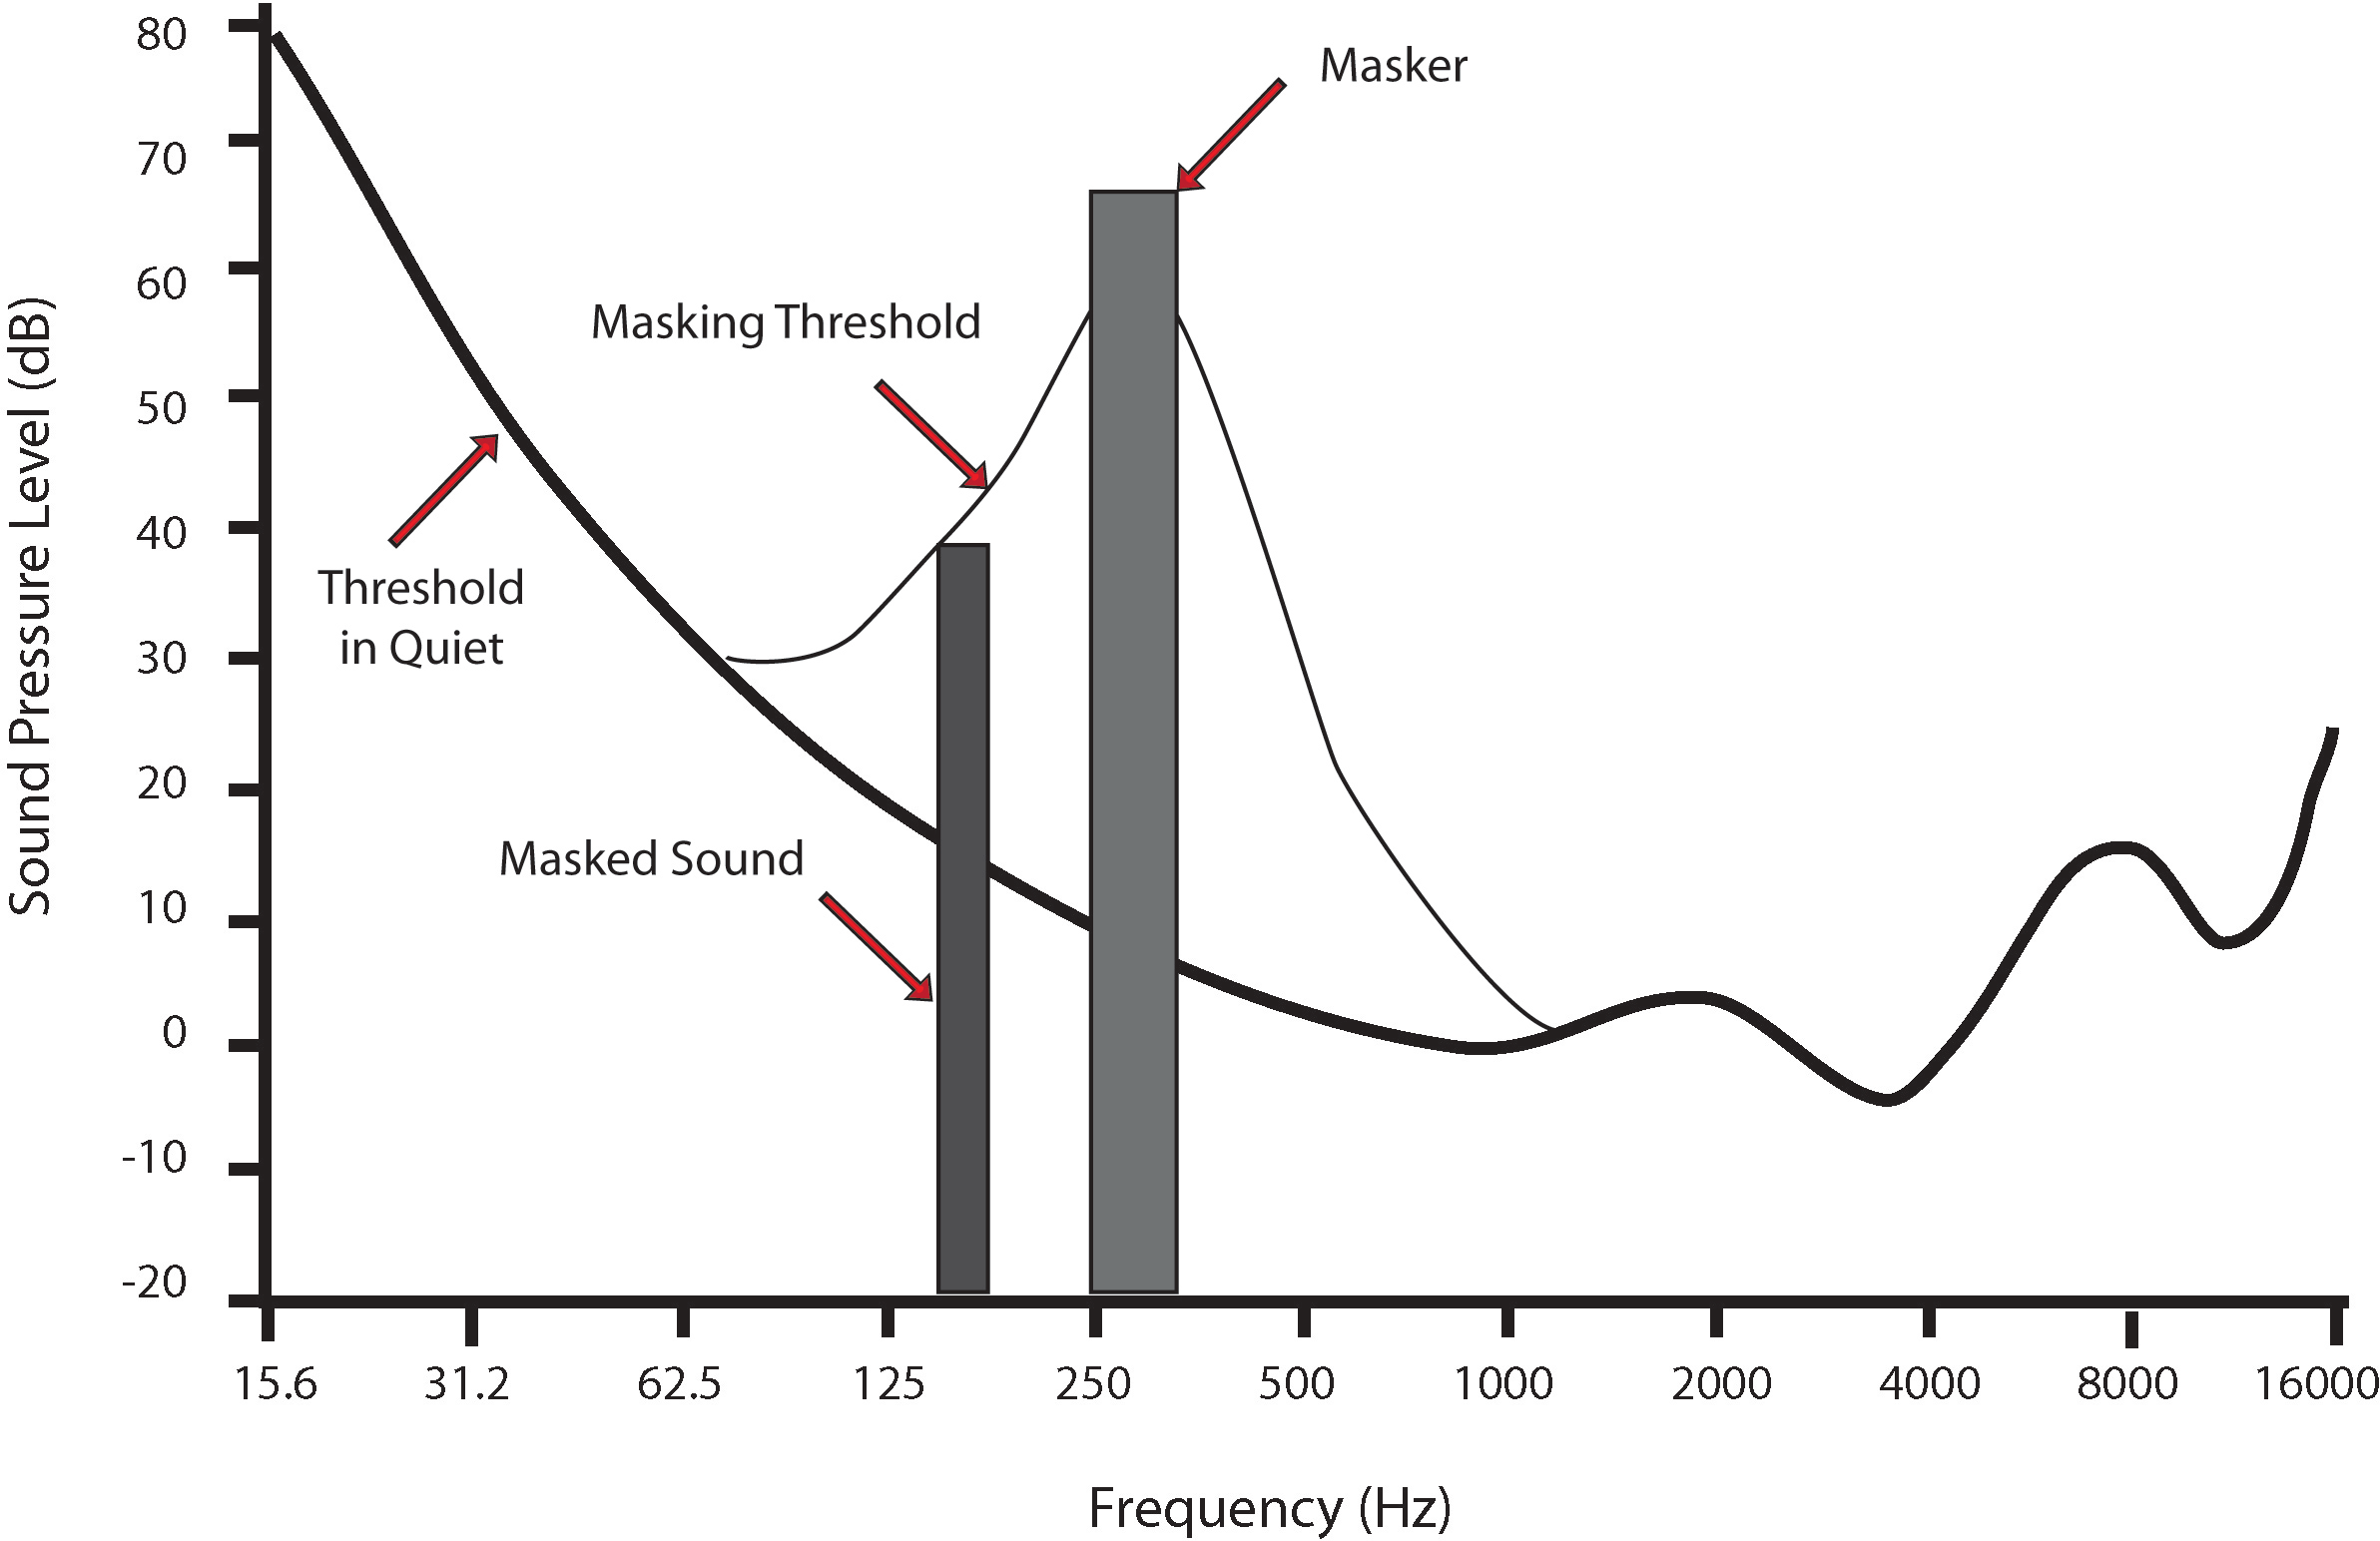
\includegraphics[width=0.7\linewidth]{files/audio-mask-graph-9e755e6993dc53c0fbb3595dc8fde6fd.png}


\textit{Image Source: \href{https://en.wikipedia.org/wiki/Masking\_(audio)}{Wikipedia - Audio Masking}}

Some real-world examples of auditory masking includes how the sound of a passing truck can mask a conversation, making it difficult to hear speech until the truck has passed. In music, masking can be used creatively to blend instruments or to hide imperfections in a recording. In \href{https://en.wikipedia.org/wiki/Hearing\_aid}{hearing aids}, understanding masking helps in designing algorithms that enhance speech while suppressing background noise.

\subsection{Shepard and Risset tones}

One of the most famous auditory illusions is named \textit{\href{https://en.wikipedia.org/wiki/Shepard\_tone}{Shepard Tones}} after \href{https://en.wikipedia.org/wiki/Roger\_Shepard}{Roger Shepard (1929--2022)}. This is a series of tones that seem to continually ascend or descend in pitch, yet never get higher or lower. This creates the auditory equivalent of a ``sonic barber pole.''

The Shepard tone is created by layering several sine waves that are spaced one octave apart. As the sequence progresses, all the sine waves move up (or down) in pitch simultaneously. The highest-pitched sine wave fades out as it reaches the top of the range, while a new, low-pitched sine wave fades in at the bottom. The overall amplitude envelope is shaped so that the listener always hears a similar blend of frequencies, with no clear starting or ending point. This continuous overlap and cross-fading trick the brain into perceiving a never-ending rise (or fall) in pitch, even though the actual frequencies are cycling within a fixed range. The illusion exploits the way our auditory system groups harmonically related tones and interprets pitch changes, making it difficult to pinpoint when the scale ``resets.''

\textit{\href{https://en.wikipedia.org/wiki/Risset\_tone}{Risset tones}}, named after French composer and scientist \href{https://en.wikipedia.org/wiki/Jean-Claude\_Risset}{Jean-Claude Risset} (1938--2016), are often confused with Shepard tones because they are similar. However, while the Shepard tones are discrete, Risset showed that it is possible to create a similar illusion also work with continuous sounds. This type of auditory illusion is similar to Shepard tones, where a continuously ascending or descending pitch seems to rise or fall endlessly. This effect is achieved by overlapping sine waves that fade in and out at different frequencies, creating the impression of a never-ending scale. Risset tones demonstrate how our perception of pitch can be manipulated by carefully controlling the spectral content and amplitude envelopes of sounds.

Both Shepard and Risset tones have been used in sound design and music. Here is one of many examples:

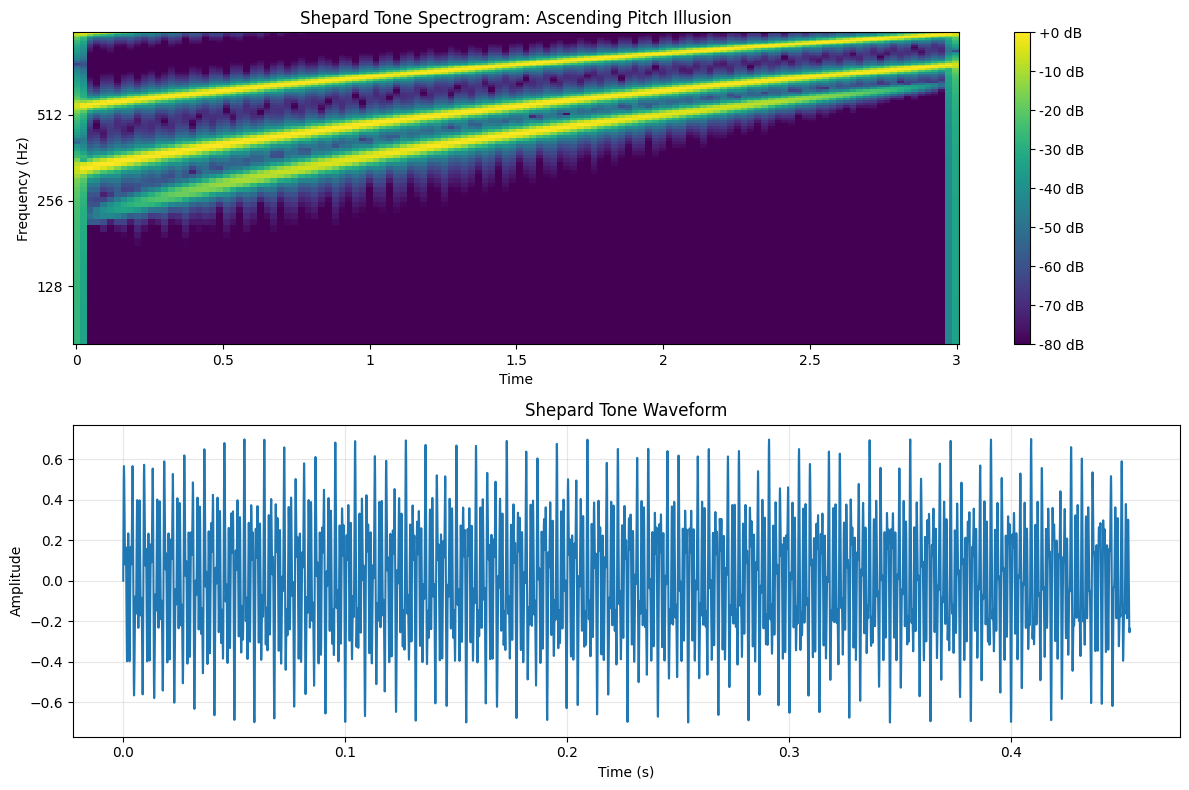
\includegraphics[width=0.7\linewidth]{files/f2307c1bc4d8b31030385c97e879a5e1.png}

\begin{verbatim}
Playing Shepard tone (3 seconds) - Notice how it seems to continuously rise!
\end{verbatim}

\subsection{Missing Fundamental}

Another powerful auditory illusion is called \textit{missing fundamental}. When a complex tone lacks its fundamental frequency but contains its harmonics, listeners still perceive the pitch corresponding to the missing fundamental. This shows that pitch perception is based on the pattern of overtones, not just the lowest frequency present.

For example, if you play a sound containing frequencies at 200 Hz, 300 Hz, and 400 Hz (the 2nd, 3rd, and 4th harmonics of 100 Hz), but omit the 100 Hz fundamental, most listeners will still perceive the pitch as if the 100 Hz tone were present. The auditory system analyzes the spacing between the harmonics and infers the fundamental frequency, even when it is physically absent.

This phenomenon is important in music and audio technology. For instance, small speakers (like those in smartphones) often cannot reproduce very low frequencies, but listeners can still perceive the intended bass notes due to the presence of higher harmonics. The missing fundamental effect is also used in telephony and audio compression to create the illusion of full-range sound with limited frequency content.

The missing fundamental illusion demonstrates that pitch perception is a constructive process, relying on the brain's ability to detect regularities and patterns in the frequency spectrum, rather than simply responding to the presence of specific frequencies.

\subsection{Binaural Beats}

When two slightly different frequencies are played separately to each ear (using headphones), the listener perceives a rhythmic beating at the frequency difference. This illusion arises from the brain's processing of phase differences between the ears.

\begin{verbatim}
- - - Missing Fundamental Illusion - - -
\end{verbatim}

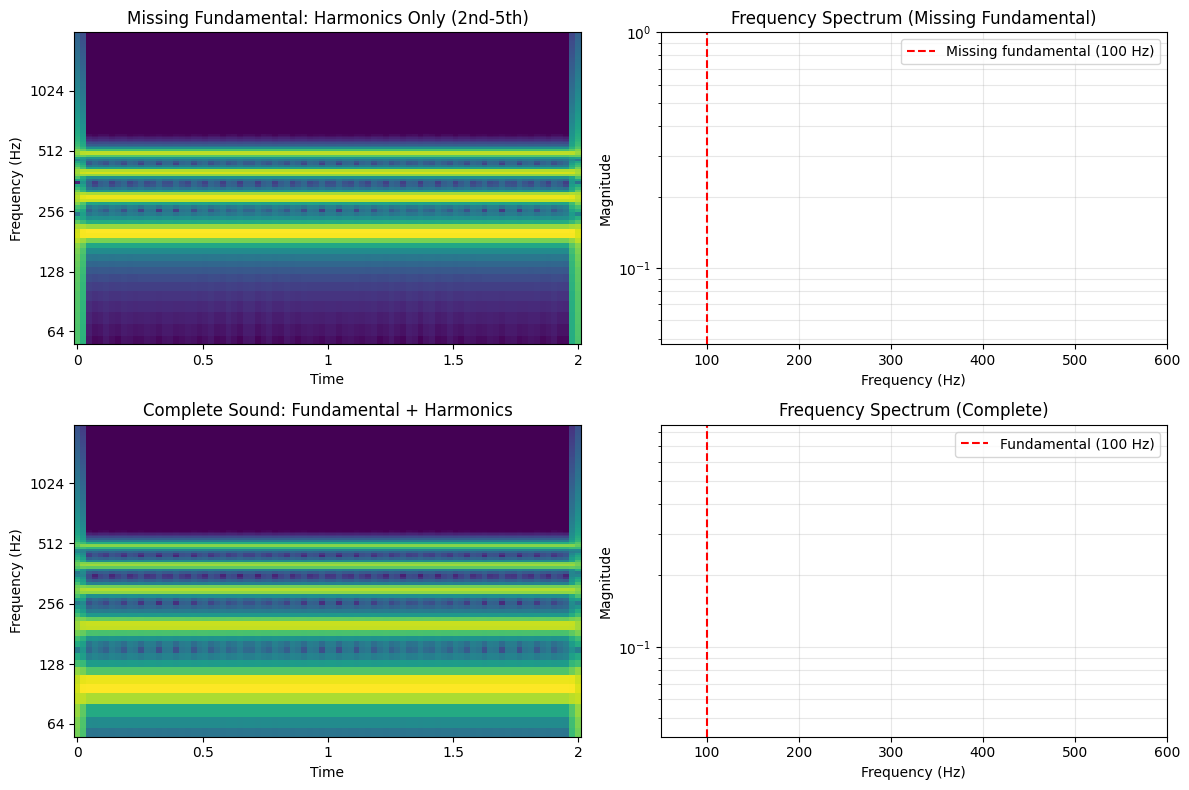
\includegraphics[width=0.7\linewidth]{files/76fae4520c04c972241560c9a159dbf5.png}

\begin{verbatim}
Both sounds should be perceived as having a pitch around 100 Hz,
even though the missing fundamental version lacks the {f_fundamental} Hz component!
\end{verbatim}

\section{Questions}

\begin{enumerate}
\item What is the difference between sound pressure level (SPL) and loudness, and why is this distinction important in psychoacoustics?


\item How does the human ear convert sound waves into electrical signals, and what are the main roles of the outer, middle, and inner ear in this process?


\item Explain the concept of masking in psychoacoustics. Give an example of how masking can affect our perception of sound in everyday life or music production.


\item What are Shepard tones and Risset tones, and how do they demonstrate the brain's role in pitch perception?


\item How do interaural time difference (ITD) and interaural level difference (ILD) help us localize sound sources in space?
\end{enumerate}


\end{document}
